% Supplementary material for the CVPR 2027 submission (built on the CVPR 2026 author kit)
\documentclass[10pt,twocolumn,letterpaper]{article}
\usepackage[review]{cvpr}
\usepackage{booktabs}
\usepackage{multirow}
\usepackage{amsmath,amssymb}
\usepackage{graphicx}
\usepackage{xcolor}
\usepackage{microtype}
%% This file contains a number of tweaks that are typically applied to the main document.
%% They are not enabled by default, but can be enabled by uncommenting the relevant lines.


%%
%% Official support for 2-column teaser figure
%%

%%
%% For auto-referencing of figures (see fig/teaser.tex and \label{} therein) 
%%
\usepackage{currfile} %< for \currfilebase macro

%%
%% caption and (global) spacing overrides
%%
\usepackage{caption} %< for "\captionof" commands (teaser)
% \setlength{\abovecaptionskip}{.5em} % space above caption
% \setlength{\belowcaptionskip}{1em} % space below caption

%%
%% Inline annotations; for predefined colors, refer to "dvipsnames" in the xcolor package:
%% https://tinyurl.com/overleaf-colors
%%
\newcommand{\red}[1]{{\color{red}#1}}
\newcommand{\todo}[1]{{\color{red}#1}}
\newcommand{\TODO}[1]{\textbf{\color{red}[TODO: #1]}}
%%
%% Disable for camera ready / submission by uncommenting these lines:
%%
% \renewcommand{\TODO}[1]{}
% \renewcommand{\todo}[1]{#1}

%%
%% Work harder in optimizing text layout. Typically shrinks text by 1/6 of page, enable
%% it at the very end of the writing process, when you are just above the page limit.
%%
% \usepackage{microtype}

%%
%% Fine-tune paragraph spacing.
%%
% \renewcommand{\paragraph}[1]{\vspace{.5em}\noindent\textbf{#1.}}

%%
%% Globally adjusts space between figure and caption.
%%
% \setlength{\abovecaptionskip}{.5em}

%%
%% Allows "the use of \paper to refer to the project name"
%% with automatic management of space at the end of the word.
%%
% \usepackage{xspace}
% \newcommand{\paper}{ProjectName\xspace}

%%
%% Commonly used math definitions.
%%
% \DeclareMathOperator*{\argmin}{arg\,min}
% \DeclareMathOperator*{\argmax}{arg\,max}

%%
%% Tighten underline.
%%
% \usepackage{soul}
% \setuldepth{foobar}

%%
%% Reconfigure paragraph (tweaks spacing)
%%

\definecolor{cvprblue}{rgb}{0.21,0.49,0.74}
\usepackage[pagebackref,breaklinks,colorlinks,allcolors=cvprblue]{hyperref}
\def\paperID{*****}
\def\confName{CVPR}
\def\confYear{2027}
\newcommand{\HI}{{\small\textsf{HI}}}
\newcommand{\MID}{{\small\textsf{MID}}}
\newcommand{\LO}{{\small\textsf{LO}}}
\newcommand{\pend}[1]{{\color{red}#1}}
\title{Supplementary Material\\When Text Locks Out Vision: Measuring Visual Headroom in Multiple-Choice VQA}
\author{Anonymous CVPR submission\\Paper ID \paperID}
\begin{document}
\maketitle
\appendix
\section{Pre-registration log}
\label{app:prereg}

Table~\ref{tab:amend} lists the amendments to the single pre-registration. Each document and each script it governs was SHA-256-hashed and timestamped before the corresponding run; amendments are appended, never edited, and cross-reference what had already been seen. ``Gate'' rows are the pre-specified checks of the original document.

\begin{table*}[h]
  \centering
  \small
  \resizebox{\textwidth}{!}{%
  \begin{tabular}{@{}l p{0.34\textwidth} p{0.50\textwidth}@{}}
    \toprule
    ID & Test & Outcome \\
    \midrule
    v1 H3 / A0, A2 & Shortest-option rule on 13{,}687 pool MCQs (range 88--94\% fixed in advance); definitions and freeze procedure & Supported: 91.90\% (CI 91.44--92.35) \\
    Gate B (validity) & Is the pool in-sample for the adapter? (confidence rule; accuracy trigger) & Pool \emph{in-sample suspected} (accuracy 98.1\%, lower bound above test); confidence rule not met; test slice not suspected \\
    Gate B/C H1 & Unadapted Qwen3.5-9B: black-image loss $\le5$ points & Not evaluable (teacher-forced readout at chance, 21.7\%) \\
    Gate C H2 & Adapter, black-image loss $\le5$ points on 700 dev MCQs & Supported: $-1.1$ points (97.0\% vs 95.9\%), in-sample suspected \\
    A3 & Replacement readout for H1 (generated answer, thinking off) & Not evaluable (2.7\% parsable; a 16-token limit was my design flaw) \\
    A4 & Qwen2.5-VL-7B, letter-only generation, true vs black image & Not evaluable (28.0\% accuracy, below the 60\% floor) \\
    A1 & Dev-split decision, retrieval design, five predictions (H4--H7) & All five supported (retrieval net $-5$; threshold from unlabeled validation) \\
    A5 & Selective prediction (transfer of the threshold, margin vs shortcut score, shortest-wrong subset) & All three supported \\
    A6, A7 & Length-equalising rewrite (two designs; gates on pass rate, manipulation, selection bias) & Both not evaluable (17.6\% and 5.2\% of questions passed; passing questions were unrepresentative) \\
    A8 & Image as tie-breaker, fresh 3{,}000 questions (C1--C6) & All six supported \\
    A9 & Controlled fine-tuning study, two public VLMs, unseen fresh questions (Sec.~4 of the main paper) & G1 (habit created) and G4 (alarm) supported for both models; G3 \emph{falsified} for both: no-veto holds (C1, C3, C4) but the image effect on undecided questions is $-1.0$ and $+1.8$ points (C2 required $\ge+5$) \\
    A10 & Recipe robustness: four single-factor variants (3 epochs, 896\,px, vision-tower LoRA, 7B with 3 epochs) & R1--R4 supported for all four: image effect on undecided questions $+2.6$, $+1.7$, $-0.7$, $-4.1$ points (none significant) \\
    A11 & Second benchmark without the length cue (PMC-VQA; Qwen 3B and 7B, InternVL3-2B) and a third family on Med-CMR; five predictions Q1\textendash{}Q5 and R1\textendash{}R5 & Med-CMR with InternVL3-2B: R1\textendash{}R5 supported. PMC-VQA: Q1 (no habit), Q2 (image gap $+13.7$ to $+14.9$ points), Q3 (undecided-stratum effect $+14.5$ to $+18.7$) supported for all three; Q5 supported on E1 and not on E2 (ratio $1.48$, $1.48$, $1.36$ against $1.5$); Q4 \emph{not evaluable} (no question has a black-image margin $\ge0.99$) \\
    A12 & Length filler (evaluation-time and training-time), counterfactual-evidence alarm combiner, saturation-aware training & L1 \emph{not evaluable} (filler costs 6--11 points); L2: models read through the filler (91\% still pick the originally shortest option); M1 (alarm) all three predictions false; M2 (weighting) false on image effect and accuracy gain \\
    A13 & Planting a length cue in PMC-VQA (three systems) & I1, I3, I4 supported (shortest 99.7\%, image gap $\approx0$ against $+14$, accuracy on original options $-14$ to $-22$ points); I2 \emph{falsified} (no question with margin $\ge0.99$) \\
    A14 & Three seeds (Qwen 3B, both benchmarks); threshold sensitivity (seven systems) & All predictions supported (Med-CMR R1--R4 and PMC-VQA Q1--Q3 for both extra seeds; T1--T3) \\
    A15 & Text--vision competition score (ten systems) and visual-strength factorial (blur) & C1 and C2 \emph{falsified} (the ratio does not beat saturation; $0/10$ held-out wins); C3 supported; F1--F3 supported for all three families \\
    A16 & 7B seeds (Med-CMR, PMC-VQA) and a third benchmark (OmniMedVQA; Qwen 3B/7B, InternVL3-2B) & S1, S2 supported; O1, O3, O4 supported; O2 (lock rule on the median margin) \emph{falsified} for all three systems \\
    A17 & Shortcut dose-response (length, six doses, three seeds), veto boundary, second shortcut (position) & H1, H2, H3a, H4, H5 and P1--P4 supported; H3b \emph{falsified} \\
    A18 & Shortcut-rescue (product-of-experts) training; training-free contrastive baseline & M-A, M-B, M-D, M-E, M-G supported; M-F (Med-CMR) \emph{falsified} (collapse to chance) \\
    A19 & Held-out transfer of the dose-response to InternVL3-2B and Qwen-7B & Rules A, B, C supported for both models (largest deviation $0.65$ and $1.96$ points; second seed in A22) \\
    A20 & Exploratory: tempered bias expert for Med-CMR & \emph{falsified}: image effect $+0.2$, $-0.2$, $-0.2$ points (required $\ge+5$ in two of three seeds); shortest-option picks 90\% \\
    A21 & Non-medical replication of the dose-response on A-OKVQA (Qwen 3B two seeds, InternVL3-2B) & R1, R3 supported in three series; R2 \emph{falsified} (accuracy on cue-free questions does not fall); R4 \emph{falsified} (benefit $+8$ to $+12$ points at $d=0.92$) \\
    A22 & Higher strengths (0.97, 0.99) and position shortcut on A-OKVQA; second seed of A19 & H1, H2, P1, P2 and S supported (lock-out reached at $d=0.99$, one seed); P3 \emph{falsified} (no boundary shift for position) \\
    A23 & Second seed of the A-OKVQA lock-out (Qwen 3B) and Qwen 7B on A-OKVQA & B1, B2, C1, C2, C3 supported (lock-out at $d=0.99$ in both) \\
    A24 & Interventions on the real Med-CMR shortcut: explicit length prior (LP), mismatched-image uniformity (MU), both (LP+MU) & criterion E1 \emph{falsified} for all three (image effect $\le+4.6$ points; LP+MU accuracy $79$--$80\%$) \\
    A25 & More seeds on A-OKVQA (Qwen 7B, InternVL3-2B, Qwen 3B) & Dose-response and boundary shift supported; lock-out at $d=0.99$ supported for Qwen 3B and 7B, \emph{falsified} for InternVL3-2B ($+1.66$ points, boundary blur 2) \\
    A26 & Second round on the real Med-CMR shortcut: gold-unlikelihood (UL), UL with the length prior, LP+MU with more seeds & UL met F1 and F2 in 3/3 seeds ($+11.6$ points against a plausible wrong image, accuracy $89.5$--$91.2\%$); LP+UL collapsed; LP+MU F1 in 4/5 seeds, F2 in none \\
    A27 & Blur test of the UL models (evaluation only) & Graded rise with image sharpness in 3/3 seeds (rule C); blur 8 recovers $\ge80\%$ of the gap in 2/3 seeds: mostly coarse image identity; LP+MU and reference flat \\
    \bottomrule
  \end{tabular}%
  }
  \caption{Pre-registered tests and outcomes (supported / falsified / not evaluable), in the order of the analysis plan, not of the run time.}
  \label{tab:amend}
\end{table*}

\section{Failed and non-evaluable tests}
\label{app:fail}

\paragraph{Base model readouts.}
Reading the answer letter from a teacher-forced position gives chance-level accuracy for the unadapted Qwen3.5-9B (21.7\% with the image, 24.9\% black), because the readout encodes the adapter's trained answer format.
A generated-answer replacement (A3) produced long descriptions that a 16-token limit cut off (2.7\% parsable); by its own rule no third readout was tried.
Zero-shot Qwen2.5-VL-7B with a letter-only prompt scored 28.0\% (black 25.5\%, below the pre-set 60\% floor) and picked the shortest option only 26\% of the time, against 91\% for the adapter, an informative contrast but not an evaluable test.

\paragraph{Length-equalising rewrites.}
Both rewrites used Qwen2.5-VL-7B as a label-blind text-only editor under frozen quality gates.
Whole-question rewriting passed 17.6\% of test questions (length violations in 78\% and altered negations in 41\% of all test questions).
Per-option rewriting with a feedback loop and character and word bands accepted 48.6\% of options but only 5.2\% of questions; the 37 that passed were already balanced (the shortest-option rule scored 62\% on them against 91\% overall).
In the data only 7\% of questions have a non-shortest correct option and the longest option is correct 28 times in 13{,}687, so a balanced subset cannot be selected; the cue can only be removed by editing, which needs a stronger editor or human edits.

\paragraph{The no-veto test on PMC-VQA.}
The pre-registered test of the no-veto property (Q4: at most 2\% of answers changed in the saturation band) could not be run because the band, a black-image margin of at least $0.99$, contains no question of the clean test set for any of the three fine-tuned models (and at most 11 of 3{,}000 for the zero-shot ones); we report the property as absent there and the answer changes under a blank image in the unsaturated strata instead (Supp.~F).

\paragraph{A falsified hypothesis.}
In the fine-tuning study (A9) the pre-registered claim that the image is worth at least $+5$ points on text-undecided questions was falsified for both public models (13 fixed against 17 broken for the 3B, 18 against 11 for the 7B), while the other three parts of that prediction held; we report it as such and do not re-run with another recipe.

\paragraph{Validity gate.}
The accuracy trigger of the development protocol (accuracy $\ge99\%$ or a Wilson lower bound above the test accuracy) fired for the pool, although pool and test margins did not differ from unseen validation questions; the margins are saturated (median 0.99997), which limits the resolution of that test.

\section{Implementation details}
\label{app:impl}

\paragraph{Readout and arms.}
Letter log-probabilities are read after the system's constant reasoning sentence and the end-of-thinking token (``direct''), softmaxed over the five letters; a second readout after the cue ``The correct option is'' behaves alike and is not used.
Black image: a $224\times224$ zero image through the system's missing-image path.
Random image: a fixed cyclic derangement within the sample.
Nearest-neighbour image: top-1 PubMedCLIP cosine similarity (mean 0.94) within the same primary modality in the retrieval corpus, excluding the case and its same-source component.
Donor images pass through the target case's modality route and preprocessing.

\paragraph{Fine-tuning study.}
Qwen2.5-VL-3B/7B-Instruct in bf16 with LoRA ($r=16$, $\alpha=32$, dropout 0.05, language-model linear layers only, fp32 adapter weights); AdamW (weight decay 0), learning rate $10^{-4}$ with 3\% warm-up and cosine decay, one epoch over 9{,}277 questions, per-device batch 1 with 16 accumulation steps, gradient clipping 1.0, seed 20261003; images downscaled to at most 448\,px; prompt with system message, image, the question with lettered options and the instruction to answer with a single letter; loss on the answer letter and the end-of-turn token only; training loss fell from 0.85 to 0.045 (3B, 27 min) and from 0.90 to 0.039 (7B, 22 min) on one H100.
Evaluation reads the five letter log-probabilities at the position after the generation prompt; each model's $\tau$ is the 15th percentile of its margins on 700 unlabeled validation questions.

\section{Reproducibility, data and licence}
\label{app:repro}

Software: PyTorch 2.7.1, Transformers 5.10.2, PEFT 0.19.1, bitsandbytes 0.49.2 on one NVIDIA H100; the baseline's FlashAttention request silently falls back to SDPA (we verified which backend loaded).
The adapter, detector and base-model shards, and all 16 code files, are byte-identical (SHA-256) to those of the released container; the container holds no training manifest.
Every Slurm job is logged with its ID, configuration, seed and output path; each amendment, script and result file has a recorded hash and timestamp, and result files were made read-only.
Data are the MedReason~2026 release, which its organisers state is governed by CC BY-NC 4.0 (research use, with attribution)~\cite{medreason2026}; we verified that the staged images are byte-identical to the public Med-CMR files and never used the 400 reserved leaderboard cases.
The later experiments (A15--A24) ran on NVIDIA A30 GPUs (24\,GB) because the H100 queue was saturated, with gradient checkpointing for the 7B and InternVL3 models, except parts H and P of A22 (A-OKVQA, Qwen 3B), which ran on NVIDIA RTX PRO 6000 Blackwell GPUs (96\,GB) with a separate PyTorch 2.7.1 environment for CUDA 12.8 (transformers 5.10.2 and peft 0.19.1 as elsewhere); A-OKVQA is used from its public release for research and no images are redistributed; OmniMedVQA (open-access subset, from the public release, images not redistributed) is licensed by its source datasets for research use.
We will release code, the amendment documents with hashes, case-id lists of all splits and samples, and the per-question prediction files (no images).

\section{Recipe-robustness variants}
\label{app:variants}

Table~\ref{tab:variants} lists all seven fine-tuned Med-CMR configurations on the same 3{,}000 unseen questions (A9, the four variants of A10, each changing one factor, and InternVL3-2B of A11).
Each model's $\tau$ is the 15th percentile of its own margins on 700 unlabeled validation questions; three epochs drive the training loss to about 0.001 and $\tau$ to about 1, which shrinks the \LO{} stratum.

\begin{table*}[h]
  \centering
  \footnotesize
  \setlength{\tabcolsep}{3pt}
  \begin{tabular}{@{}lccrrcrc@{}}
    \toprule
    Configuration & \LO{} $n$ & \LO{} effect (pts, $p$) & \HI{} chg. & Gap & Short. (test) & Errors flagged & Acc. \\
    \midrule
    A9: 3B, 1 epoch, 448\,px         & 410 & $-1.0$ (0.58) & 0/2518 & $-0.1$ & 92.3\% & 131/135 & 95.5\% \\
    A9: 7B, 1 epoch, 448\,px         & 386 & $+1.8$ (0.26) & 0/2503 & $+0.2$ & 91.7\% & 118/120 & 96.0\% \\
    V1: 3B, 3 epochs                 & 152 & $+2.6$ (0.54) & 0/2499 & $+0.2$ & 91.8\% & 119/125 & 95.8\% \\
    V2: 3B, 896\,px                  & 424 & $+1.7$ (0.23) & 0/2530 & $+0.2$ & 91.7\% & 123/126 & 95.8\% \\
    V3: 3B, vision-tower LoRA        & 404 & $-0.7$ (0.68) & 0/2533 & $-0.1$ & 92.0\% & 135/138 & 95.4\% \\
    V4: 7B, 3 epochs                 & 147 & $-4.1$ (0.31) & 0/2472 & $-0.3$ & 92.3\% & 121/123 & 95.9\% \\
    A11: InternVL3-2B, 1 epoch      & 461 & $-0.2$ (1.0)  & 0/2514 & $0.0$  & 91.1\% & 153/154 & 94.9\% \\
    \midrule
    Released adapter (A8)$^\ddagger$ & 239 & $+12.1$ ($1.5\!\times\!10^{-5}$) & 0/2463 & $+1.1$ & 91\% & 52/52 & 98.3\% \\
    \bottomrule
  \end{tabular}
  \caption{\textbf{All fine-tuned configurations.} The prediction of A10 (image effect on undecided questions below $+5$ points) held in every variant. ``Gap'' is accuracy with the true minus with a black image over all 3{,}000 questions; ``Short.'' the share of test predictions equal to the shortest option; ``Acc.'' fresh accuracy. $^\ddagger$ In-sample suspected.}
  \label{tab:variants}
\end{table*}

\section{PMC-VQA study (A11)}
\label{app:pmc}

Data: PMC-VQA \cite{zhang2023pmcvqa}, the official clean test set (E1, 1{,}999 usable questions of 2{,}000; one row has duplicated options), 3{,}000 held-out train-file questions (E2), 700 unlabeled validation questions (setting each model's $\tau_m$), and 9{,}277 training questions; all four sets are disjoint by source article, and train articles occurring in the test set were removed. Counterfactual images: black, a random other-article image, and the PubMedCLIP nearest neighbour from another article (no modality restriction). The recipe is that of A9 (Sec.~4 of the main paper) with four letters; training took 27, 22 and 28 minutes (loss \textrm{0.73--0.91}\ to 0.54--0.56).
Because margins are far from saturated here ($\tau_m\approx0.04$), the strata of Sec.~3 of the main paper do not isolate decisive text, and the paper's conclusions rest on the all-question gap, the undecided stratum, and the saturation band, which is empty.

\begin{table*}[h]
  \centering
  \footnotesize
  \setlength{\tabcolsep}{3pt}
  \begin{tabular}{@{}lccccccccccrr@{}}
    \toprule
    Model & Zero-shot & FT & FT black & Gap & \LO{} eff. & $\tau_m$ & \HI{} chg. & Short. & Err. ratio & AUROC & Flag./capt. & Gap E2 \\
    \midrule
    Qwen2.5-VL-3B & 50.2 & 51.8 & 38.1 & $+13.7$ & $+14.5$ & 0.039 & 30.6\% & 25.1\% & 1.50 & 0.72 & 13.3\% / 18.7\% & $+12.9$ \\
    Qwen2.5-VL-7B & 52.2 & 54.1 & 39.2 & $+14.9$ & $+18.1$ & 0.042 & 30.0\% & 24.3\% & 1.76 & 0.76 & 14.2\% / 22.5\% & $+12.6$ \\
    InternVL3-2B & 49.0 & 51.0 & 36.6 & $+14.4$ & $+18.7$ & 0.038 & 30.3\% & 27.4\% & 1.60 & 0.73 & 13.3\% / 19.7\% & $+9.8$ \\
    \bottomrule
  \end{tabular}
  \caption{\textbf{PMC-VQA, clean test set (E1), fine-tuned systems.} Accuracy (\%) zero-shot and after fine-tuning (FT) with the true and with a black image; ``Gap'' and ``\LO{} eff.'' are accuracy with the true minus with a black image over all questions and in the least-confident stratum (points; all $p<10^{-5}$); ``\HI{} chg.'' the share of answers in the $m_b\ge\tau_m$ stratum that change under a black image; ``Short.'' the share of predictions equal to the unique shortest option (the correct option is it in 19.7\%); ``Err. ratio'' the error rate of flagged over unflagged questions and ``AUROC'' that of the margin for errors; ``Flag./capt.'' the flagged share of questions and the share of errors it contains; ``Gap E2'' the all-question gap on the 3{,}000 held-out questions.}
  \label{tab:pmc}
\end{table*}

\section{Fine-tuning study on Med-CMR (A9)}
\label{app:ft}

Table~4 gives the full comparison of the released adapter and the two fine-tuned Qwen2.5-VL models on the same protocol (Sec.~4 of the main paper).

\begin{table*}[h]
  \centering
  \small
  \setlength{\tabcolsep}{8pt}
  \begin{tabular}{@{}lccc@{}}
    \toprule
     & Adapter & FT 3B & FT 7B \\
    \midrule
    Test accuracy, before $\to$ after (\%) & -- $\to$ 96.1 & 24.5 $\to$ 95.4 & 27.7 $\to$ 95.4 \\
    Test: shortest option, before $\to$ after (\%) & -- $\to$ 91 & 23 $\to$ 92 & 25 $\to$ 92 \\
    Fresh accuracy (\%) & 98.3$^\ddagger$ & 95.5 & 96.0 \\
    Fresh \#questions \HI{}/\MID{}/\LO{} & 2463/298/239 & 2518/72/410 & 2503/111/386 \\
    \HI{}: answers changed by any wrong image & 0 & 0 & 0 \\
    \LO{}: image effect, points ($p$) & $+12.1$ ($1.5\!\times\!10^{-5}$) & $-1.0$ (0.58) & $+1.8$ (0.26) \\
    \LO{}: accuracy change with a random image, points & $-11.7$ & $+0.7$ & $-5.4$ \\
    Headline gap, points & $+1.1$ & $-0.1$ & $+0.2$ \\
    Errors in the flagged 16\% & 52/52 & 131/135 & 118/120 \\
    \bottomrule
  \end{tabular}
  \caption{\textbf{Three systems, same protocol.} ``Before'' is zero-shot with the same readout (the adapter has no zero-shot state). Image effect = accuracy with the true minus with a black image; random-image row = accuracy with a random image minus with the true image. $^\ddagger$ In-sample suspected.}
  \label{tab:train}
\end{table*}

\section{Error alarm and risk--coverage}
\label{app:alarm}

Table~5 and Fig.~1 give the pre-registered error alarm of the released adapter on the four labelled samples (summarised in Sec.~4 of the main paper).

\begin{table}[h]
  \centering
  \small
  \setlength{\tabcolsep}{3.0pt}
  \begin{tabular}{@{}lrrrrr@{}}
    \toprule
    Sample & $n$ & Errors & Flagged & Caught & Answered right \\
    \midrule
    Fresh (A8)   & 3000 & 52 & 16.4\% & 52/52 & 2507/2507 \\
    Dev          &  700 & 21 & 15.1\% & 21/21 &  594/594 \\
    Pool         &  700 & 13 & 15.1\% & 13/13 &  594/594 \\
    Test$^\dagger$ &  711 & 28 & 15.8\% & 28/28 &  599/599 \\
    \bottomrule
  \end{tabular}
  \caption{\textbf{The error alarm at the pre-registered threshold.} Fresh, dev and pool are in-sample suspected for the adapter; $^\dagger$ exploratory.}
  \label{tab:alarm}
\end{table}

\begin{figure*}[h]
  \centering
  \includegraphics[width=\textwidth]{fig/f4_risk_coverage.pdf}
  \caption{\textbf{Risk--coverage.} Accuracy of the answered questions when the least confident ones are skipped (coverage from 100\% to 40\%), against random skipping.}
  \label{fig:rc}
\end{figure*}

\section{Released adapter: where the image matters (A8)}
\label{app:teaser}

Figure~\ref{fig:where} shows the released adapter on 3{,}000 fresh questions that no earlier analysis had touched (in-sample suspected, see the main text).
In the text-decisive stratum (82\% of the questions) no counterfactual image, whether black, random or a similar wrong one, changed any of 2{,}463 answers; in the text-undecided stratum (8\%) the image is worth $+12.1$ points (exact McNemar $p=2\times10^{-5}$); over all questions the gap is $1.1$ points.

\begin{figure*}[h]
  \centering
  \includegraphics[width=\textwidth]{fig/f1_where_image_matters.pdf}
  \caption{\textbf{Where the image matters, for the released adapter.} (a)~Accuracy with the true and with a black image by text-saturation stratum (\HI{}: margin $\ge0.995$). (b)~Share of questions per stratum (top) and share of all prediction changes without the image (bottom): 94\% of them occur in the 8\% of questions where the text is undecided.}
  \label{fig:where}
\end{figure*}

\section{Length intervention, alarm combiner and saturation-aware training (A12)}
\label{app:a12}

\paragraph{Filler intervention.}
Every option is extended by neutral adverbs (``often'', ``typically'', ``especially'', \dots) so that the five final lengths are exactly $s_{\max}+4j$ characters; in \emph{pres} the original length order is kept, in \emph{rand} the length rank of each option is a random permutation (the correct option is the shortest in 20\% of questions).
Table~\ref{tab:l1} shows the evaluation-time test on the A9 models and Table~\ref{tab:l2} the models trained on \emph{rand} options.
The filler alone costs 6--11 points (V failed, so L1 is not evaluable), and under \emph{rand} the models follow the originally shortest option, not the padded one.

\begin{table}[h]
  \centering
  \footnotesize
  \setlength{\tabcolsep}{2.5pt}
  \resizebox{\columnwidth}{!}{%
  \begin{tabular}{@{}llcccc@{}}
    \toprule
    Model & Condition & Test acc. & Fresh acc. & = padded shortest & = original shortest \\
    \midrule
    Qwen 3B & orig & 95.4 & 95.5 & 91.0 & 91.0 \\
            & pres & 85.4 & 84.2 & 83.7 & 82.6 \\
            & rand & 80.5 & 77.1 & 24.5 & 77.1 \\
    Qwen 7B & orig & 95.4 & 96.0 & 90.6 & 90.6 \\
            & pres & 89.2 & 89.9 & 87.8 & 86.2 \\
            & rand & 85.2 & 83.8 & 24.2 & 81.6 \\
    \bottomrule
  \end{tabular}%
  }
  \caption{\textbf{Evaluation-time intervention (L1).} Accuracy (\%) of the A9 fine-tuned models on the test and fresh questions with original options, with filler that preserves the length order (pres), and with randomised length ranks (rand); share of test predictions equal to the padded and to the originally shortest option.}
  \label{tab:l1}
\end{table}

\begin{table}[h]
  \centering
  \footnotesize
  \setlength{\tabcolsep}{2.5pt}
  \resizebox{\columnwidth}{!}{%
  \begin{tabular}{@{}lcccccc@{}}
    \toprule
    Model & Acc. & = pad.\ sh. & = orig.\ sh. & $m_b\!\ge\!.99$ & Gap (p) & \LO{} eff. \\
    \midrule
    Qwen 3B & 95.1 & 18.4 & 90.7 & 77.7 & $+0.4$ (0.058) & $+2.9$ (n 415) \\
    Qwen 7B & 95.7 & 18.7 & 90.9 & 78.6 & $+0.2$ (0.30) & $+1.8$ (n 395) \\
    \bottomrule
  \end{tabular}%
  }
  \caption{\textbf{Training on randomised length ranks (L2).} Fresh accuracy (\%), share of test predictions equal to the padded-shortest and to the originally shortest option, share of fresh questions with a black-image margin $\ge0.99$, all-question image gap and effect in the least-confident stratum.}
  \label{tab:l2}
\end{table}

\paragraph{Counterfactual-evidence alarm (M1).}
A logistic combiner (C=1) of eight features (true and black margins, JS divergence between true- and black-image distributions, agreement with and divergence from the random- and nearest-neighbour-image predictions, top-1 probability) is fitted on PMC-VQA E2 and tested on E1, and cross-fitted by case-id parity on Med-CMR.
AUROC against the margin alone: PMC-VQA $0.724$ vs $0.716$ (Qwen 3B), $0.760$ vs $0.755$ (7B), $0.725$ vs $0.727$ (InternVL); Med-CMR $0.950$ vs $0.965$, $0.966$ vs $0.968$, $0.962$ vs $0.969$.
The share of errors in the 15\% highest scores changes by $+0.1$, $0.0$, $-0.9$ points (PMC-VQA) and $-1.5$, $0.0$, $-0.7$ (Med-CMR).

\paragraph{Saturation-aware training (M2).}
Two text-only bias models (Qwen 3B, black image, A9 recipe, each trained on one half of the training questions) score the other half; the 14.5\% of training questions with a text-only margin below 0.90 get loss weight 1, the others 0.25.
On the 410 fresh questions that are undecided for the A9 3B model the image effect is $+1.46$ points (17 fixed, 11 broken, $p=0.34$) against $-0.98$ for A9, accuracy with the image $69.0\%$ against $68.5\%$; overall fresh accuracy $95.57\%$ against $95.50\%$; shortest-option share 90.9\%.


\section{Planting a length cue in PMC-VQA (A13)}
\label{app:a13}

Neutral filler is added to all four options so that the final lengths are $s_{\max}+4j$ characters; the correct option receives the shortest length with probability 0.92 (realised: 91.8\% on E1) and a random other rank otherwise.
The three systems are fine-tuned with the A11 recipe on the planted training questions and evaluated with true and black images on planted E1, planted E2 and original E1 (Table~\ref{tab:a13}).

\begin{table}[h]
  \centering
  \footnotesize
  \setlength{\tabcolsep}{2.5pt}
  \resizebox{\columnwidth}{!}{%
  \begin{tabular}{@{}lccc@{}}
    \toprule
     & Qwen 3B & Qwen 7B & InternVL 2B \\
    \midrule
    A11 (original options): E1 accuracy / gap & 51.8 / $+13.7$ & 54.1 / $+14.9$ & 51.0 / $+14.4$ \\
    Planted E1: accuracy (black) & 91.7 (91.7) & 91.8 (91.9) & 91.8 (91.6) \\
    Planted E1: gap ($p$) & $+0.05$ (1.0) & $-0.10$ (0.63) & $+0.20$ (0.13) \\
    Planted E1: prediction = shortest & 99.7 & 99.8 & 99.6 \\
    Planted E1: black margin $\ge0.99$ / $\ge0.5$ & 0 / 99.3 & 0 / 99.8 & 0 / 98.9 \\
    Planted E2: gap & $-0.13$ & $-0.10$ & $0.00$ \\
    Original E1: accuracy (black) & 38.2 (27.5) & 38.8 (27.1) & 28.6 (24.6) \\
    Original E1: gap & $+10.7$ & $+11.7$ & $+3.95$ \\
    \bottomrule
  \end{tabular}%
  }
  \caption{\textbf{Planted length cue on PMC-VQA (A13).} Percentages unless stated; ``gap'' is accuracy with the true minus with a black image in points. Predictions I1, I3 and I4 held for all three systems; I2 (at least 30\% of questions with a black-image margin $\ge0.99$) did not.}
  \label{tab:a13}
\end{table}


\section{Retrieval of similar cases (A1)}
\label{app:retr}

The adapter was built to be improved by retrieval, so we tested it: for each of the 711 test MCQs we retrieved the three most similar training cases in the same modality (PubMedCLIP image embeddings, corpus without same-source cases) and put their questions and verified answers into the prompt.
Accuracy fell from 683 to 678 correct (net $-5$, $p=0.30$); three random same-modality neighbours gave 680 ($-3$), so the loss is a prompt-format effect, not retrieval; retrieving from the full pool with same-source cases (the index finds the partner in 36 of 47 cases) gave 679 ($-4$); applying retrieval only to the low-margin cases gave 678 ($-5$); and with the image blacked out retrieval did not substitute for it (673 against 677).
All five pre-registered predictions held.
This agrees with a related preprint reporting that changing the number of in-prompt examples moves accuracy by at most one case once its adapter is fixed~\cite{kirscher2026optionaware}; we tested one encoder, $k=3$, one prompt and one model trained on this distribution, so we do not claim that retrieval cannot help any model.

\section{Fresh-data test of the tie-breaker structure (A8)}
\label{app:a8}

\begin{table}[h]
  \centering
  \footnotesize
  \setlength{\tabcolsep}{2.4pt}
  \begin{tabular}{@{}lrrrrrr@{}}
    \toprule
     & & \multicolumn{2}{c}{Accuracy (\%)} & Fix/ & \multicolumn{2}{c}{Changed, \#} \\
    \cmidrule(lr){3-4}\cmidrule(l){6-7}
    Stratum & $n$ & true & black & break & black & wrong img \\
    \midrule
    \HI{} (text decides) & 2463 & 100.0 & 100.0 & 0/0 & 0 & 0 \\
    \MID{}               &  298 &  99.3 &  98.3 & 3/0 & 3 & 5 \\
    \LO{} (undecided)    &  239 &  79.1 &  67.0 & 37/8 & 49 & 55 \\
    \midrule
    All                  & 3000 &  98.3 &  97.2 & 40/8 & 52 & 60 \\
    \bottomrule
  \end{tabular}
  \caption{\textbf{Fresh-data test (A8).} Fix/break: questions the true image gets right and the black image wrong, and the reverse. ``Wrong img'': prediction changes with a similar but wrong image.}
  \label{tab:a8}
\end{table}

\section{Option-length dose--response}
\label{app:dose}

\begin{figure}[h]
  \centering
  \includegraphics[width=0.6\columnwidth]{fig/f2_length_dose_response.pdf}
  \caption{\textbf{Accuracy falls as the length cue weakens} (711 test MCQs, exploratory). Accuracy of the adapter with the true and the black image, binned by the length of the correct option over the mean length of the wrong options.}
  \label{fig:dose}
\end{figure}

\section{Seeds and threshold sensitivity (A14)}
\label{app:a14}

\begin{table}[h]
  \centering
  \footnotesize
  \setlength{\tabcolsep}{2.2pt}
  \begin{tabular}{@{}llccccc@{}}
    \toprule
    Benchmark & Seed & Gap & \LO{} effect & Shortest & \HI{} chg. & Caught \\
    \midrule
    Med-CMR & 0 & $-0.13$ & $-0.98$ (0.58) & 92.3 & 0/2518 & 131/135 \\
            & 1 & $-0.03$ & $-0.24$ (1.0)  & 92.1 & 0/2528 & 134/137 \\
            & 2 & $+0.13$ & $+1.06$ (0.52) & 92.0 & 0/2510 & 131/135 \\
    PMC-VQA & 0 & $+13.7$ & $+14.5$ & 25.1 & -- & 18.7\% \\
            & 1 & $+15.3$ & $+16.9$ & 24.4 & -- & 19.7\% \\
            & 2 & $+14.1$ & $+18.1$ & 24.8 & -- & 22.0\% \\
    \bottomrule
  \end{tabular}
  \caption{\textbf{Three seeds of the Qwen2.5-VL-3B recipe on each benchmark.} Gap: accuracy with the true minus with a black image over all questions (points); \LO{} effect in the least-confident stratum (points, McNemar $p$ on Med-CMR; all $p<10^{-3}$ on PMC-VQA); shortest: share of test (Med-CMR) or E1 (PMC-VQA) predictions equal to the shortest option; \HI{} chg.: text-decisive answers changed by a black image; caught: errors in the flagged questions. Means (sd): Med-CMR gap $-0.01$ (0.13), \LO{} effect $-0.05$ (1.03); PMC-VQA gap $14.3$ (0.83), \LO{} effect $16.5$ (1.8).}
  \label{tab:seeds-app}
\end{table}

\begin{figure*}[t]
  \centering
  \includegraphics[width=0.85\textwidth]{fig/f6_threshold.pdf}
  \caption{\textbf{Threshold sensitivity on Med-CMR.} (a)~Image effect (true minus black accuracy) in the questions whose black-image margin is below a cut-off (numbers: questions for the released adapter). (b)~Share of answers changed by a black image among the questions with a margin above a cut-off. The fine-tuned models stay below the $+5$-point line at every cut-off; the released adapter's effect grows as the cut-off tightens; no answer changes at cut-offs of 0.99 and above.}
  \label{fig:thr}
\end{figure*}

\section{Competition score and visual-strength factorial (A15)}
\label{app:a15}

\paragraph{Competition score.}
For each question, $M_T$ is the log-odds margin of the black-image answer $a^*$; $\Delta(I')$ is how far an image $I'$ moves the log-odds against $a^*$; $\Delta_{\rm wrong}$ is the larger of $\Delta$ for the random and the nearest-neighbour image; the competition ratio is $R=\Delta_{\rm wrong}/(M_T+0.1)$.
These wrong-image quantities are used to predict whether the \emph{true} image overrides $a^*$ (a prediction that cannot be true by construction).
Table~\ref{tab:a15c} gives the AUROC of text saturation, of $R$ and of the deficit $\Delta_{\rm wrong}-M_T$ (exploratory), and the leave-one-system-out log-loss.
Pre-registered C1 (the ratio beats the best text score by 0.02 in at least 70\% of the evaluable systems) and C2 (lower leave-one-system-out log-loss in at least 8 of 10 systems) both failed.

\begin{table}[h]
  \centering
  \footnotesize
  \setlength{\tabcolsep}{2.2pt}
  \resizebox{\columnwidth}{!}{%
  \begin{tabular}{@{}llrrrrrr@{}}
    \toprule
    Data & System & Overr. & Sat. & Ratio & Deficit & LL text & LL add. \\
    \midrule
    Med-CMR & Adapter & 52 & .978 & .943 & .985 & .052 & .047 \\
            & Qwen 3B & 40 & .987 & .942 & .991 & .034 & .028 \\
            & Qwen 7B & 33 & .983 & .948 & .994 & .032 & .025 \\
            & InternVL & 44 & .983 & .904 & .993 & .040 & .032 \\
    PMC-VQA & Qwen 3B & 772 & .697 & .767 & .790 & .620 & .559 \\
            & Qwen 7B & 743 & .692 & .732 & .753 & .606 & .573 \\
            & InternVL & 749 & .683 & .788 & .810 & .622 & .541 \\
    Planted & 3 systems & 4--10 & \multicolumn{5}{c}{not evaluable (fewer than 40 overrides)} \\
    \bottomrule
  \end{tabular}%
  }
  \caption{\textbf{Predicting visual overrides (A15).} Overr.: questions whose answer under the true image differs from the black-image answer. AUROC of text saturation (Sat.), of the pre-registered competition ratio (Ratio) and of the exploratory deficit; LL: leave-one-system-out log-loss of a logistic model on the text margin (text) and on the text margin plus wrong-image evidence (add.). The ratio is below saturation on Med-CMR (C1 and C2 failed); the additive model has the lower log-loss in 9 of 10 systems.}
  \label{tab:a15c}
\end{table}

\paragraph{Visual-strength factorial.}
Table~\ref{tab:a15f} gives accuracy as the true image is replaced by a black image, a blurred image (radius 24 and 8\,px) and the intact image (A30 GPUs, evaluation only).

\begin{table}[h]
  \centering
  \footnotesize
  \setlength{\tabcolsep}{2.2pt}
  \begin{tabular}{@{}llrrrr@{}}
    \toprule
    Text condition & Family & Black & Blur 24 & Blur 8 & True \\
    \midrule
    PMC-VQA & Qwen 3B & 38.4 & 39.0 & 40.5 & 51.5 \\
            & Qwen 7B & 39.9 & 40.5 & 42.2 & 54.2 \\
            & InternVL & 36.8 & 36.4 & 39.3 & 50.9 \\
    Planted cue & Qwen 3B & 91.6 & 91.7 & 91.6 & 91.7 \\
            & Qwen 7B & 91.9 & 91.9 & 91.8 & 91.8 \\
            & InternVL & 91.6 & 91.7 & 91.7 & 91.7 \\
    Med-CMR & Qwen 3B & 95.6 & 95.6 & 95.6 & 95.5 \\
            & Qwen 7B & 95.8 & 95.7 & 95.8 & 96.0 \\
            & InternVL & 94.9 & 95.0 & 95.0 & 95.0 \\
    \bottomrule
  \end{tabular}
  \caption{\textbf{Accuracy (\%) by visual evidence strength and text condition (A15).} The image benefit grows with visual strength only on PMC-VQA; with a locked text (planted cue, Med-CMR) it is within $\pm0.3$ points at every strength. Predictions F1--F3 held for all three families.}
  \label{tab:a15f}
\end{table}


\section{Dose-response and the visual veto boundary (A17)}
\label{app:dose17}

Qwen2.5-VL-3B, PMC-VQA, the A11 recipe; the length shortcut planted with neutral filler on all options at strength $d$ (rank-based assignment: realised cue rate equals $d$ to within one question; nested across doses; $d=0.25$ is the filler control); three seeds (20261011--13) for each of the six doses and one seed for the answer-position shortcut at three doses; evaluation on the 1{,}999 clean test questions with true, black, random, nearest-neighbour and degraded images (Gaussian blur radius 32, 16, 8, 4, 2\,px; downsampling to 8--128\,px for $d\in\{0.25,0.70,0.92\}$ in one seed).
Table~\ref{tab:dose17} gives the per-dose results, Table~\ref{tab:h17} the pre-registered tests, Fig.~\ref{fig:s_dose} the shortcut habit and the text margin, and Figs.~\ref{fig:s_phase}--\ref{fig:s_second} the override map, the boundary and the second shortcut.
The veto boundary $V^\ast$ is the weakest ladder level (1 = blur 32, \dots, 6 = intact) at which the image benefit is at least $+2.0$ points with a paired-bootstrap lower bound of at least $+1.0$; 7 means that no level qualifies.

\begin{table*}[h]
  \centering
  \footnotesize
  \setlength{\tabcolsep}{4pt}
  \resizebox{\textwidth}{!}{%
  \begin{tabular}{@{}rcccccccc@{}}
    \toprule
    $d$ (\%) & $g$(intact), mean (sd) & $V^\ast$ (3 seeds) & Shortest pick (\%) & Median $M_T$ & Acc.\ true / black (\%) & Cue-free acc.\ (\%) & Override (\%) \\
    \midrule
    25 & 13.5 (0.5) & 4,3,3 & 22 & 0.29 & 50.8 / 37.4 & 51.9 & 39.4 \\
    40 & 13.2 (0.7) & 3,4,4 & 41 & 0.33 & 52.8 / 39.6 & 50.0 & 36.9 \\
    55 & 8.0 (0.6) & 5,4,5 & 75 & 0.79 & 60.6 / 52.6 & 46.5 & 19.9 \\
    70 & 3.4 (0.2) & 5,5,5 & 93 & 1.67 & 72.1 / 68.8 & 42.9 & 6.9 \\
    85 & 0.4 (0.2) & 7,7,7 & 99 & 2.58 & 85.0 / 84.6 & 40.4 & 1.2 \\
    92 & 0.1 (0.1) & 7,7,7 & 100 & 3.21 & 91.7 / 91.6 & 38.1 & 0.3 \\
    \bottomrule
  \end{tabular}%
  }
  \caption{\textbf{Shortcut dose-response (A17; three seeds, Qwen2.5-VL-3B, PMC-VQA E1).} $g$(intact): image benefit of the intact image (points); $V^\ast$: veto boundary by seed; shortest pick: share of predictions equal to the shortest option; median $M_T$: median black-image log-odds margin; accuracies on the matched (planted) test; cue-free acc.: accuracy on the original, unplanted options; override: share of intact-image predictions that differ from the black-image answer.}
  \label{tab:dose17}
\end{table*}

\begin{table}[h]
  \centering
  \footnotesize
  \setlength{\tabcolsep}{3pt}
  \resizebox{\columnwidth}{!}{%
  \begin{tabular}{@{}lll@{}}
    \toprule
    Test & Statistic & Result \\
    \midrule
    H1 benefit vs dose & $\rho=-0.963$, $p<10^{-4}$ & supported \\
    H2 boundary vs dose & $\rho=+0.943$ & supported \\
    H3a margin vs dose & $\rho=+0.975$ & supported \\
    H3b margin as predictor & RMSE 1.66 vs 1.22 (limit 1.53) & \emph{not supported} \\
    H4 override vs dose & $\rho=-0.988$ & supported \\
    H5 downsampling ladder & $V^\ast$: 3, 5, none & supported \\
    P1--P4 position shortcut & $g=+17.8,+6.4,0.0$; $V^\ast=3,5,7$ & supported \\
    \bottomrule
  \end{tabular}%
  }
  \caption{\textbf{Pre-registered tests of A17.} Permutation $p$-values (10{,}000 permutations of the dose within seeds), Holm-corrected over H1--H4.}
  \label{tab:h17}
\end{table}

\begin{figure*}[h]
  \centering
  \includegraphics[width=0.95\textwidth]{fig/f7_dose_response.pdf}
  \caption{\textbf{Shortcut dose-response on PMC-VQA} (Qwen2.5-VL-3B, three seeds; thin lines: seeds). (a)~Image benefit of the intact image; dashed: the answer-position shortcut (one seed). (b)~Share of predictions equal to the shortest option. (c)~Median text margin with a black image (log-odds).}
  \label{fig:s_dose}
\end{figure*}

\begin{figure*}[h]
  \centering
  \includegraphics[width=0.95\textwidth]{fig/f7_phase_diagram.pdf}
  \caption{\textbf{Image benefit and override rate by shortcut strength and visual strength} (mean of three seeds).}
  \label{fig:s_phase}
\end{figure*}

\begin{figure*}[h]
  \centering
  \includegraphics[width=0.95\textwidth]{fig/f7_boundary_shift.pdf}
  \caption{\textbf{The veto boundary and the text margin.} (a)~$V^\ast$ against the dose. (b)~Image benefit against the median text margin (blue: $d\le0.55$; orange: $d\ge0.70$).}
  \label{fig:s_boundary}
\end{figure*}

\begin{figure*}[h]
  \centering
  \includegraphics[width=0.95\textwidth]{fig/f7_second_shortcut.pdf}
  \caption{\textbf{Second shortcut (answer position).} (a)~Image benefit against the dose for both shortcuts. (b)~Ladders for the position shortcut at three doses.}
  \label{fig:s_second}
\end{figure*}


\section{Shortcut-rescue training (A18, A20)}
\label{app:rescue}

A text-only bias expert (Qwen2.5-VL-3B, black image, A11 recipe) is trained on one half of the training questions and scores the other half; the main model is trained on $\log p_{\rm main}+\ell_b$ (weight 1) and used alone at test time; the control uses the same letter-restricted loss with weight 0.
The experts' cross-fitted accuracy is 91.5\% and 91.9\% (folds A, B) at $d=0.92$ and 68.1\% and 70.4\% at $d=0.70$, i.e.\ they have learned the shortcut from other questions.
Table~\ref{tab:rescue} gives each run and Fig.~\ref{fig:rescue} the visual ladder and the accuracies; the naive models of the same doses are in Table~\ref{tab:dose17}.
On Med-CMR the rescue models collapse to chance accuracy (19.8\%, 21.3\%, 21.5\%; A9: 95.5\%) because the A12 expert is saturated (median margin $0.9995$) and gives the main model almost no gradient (M-F not supported).
A20 (exploratory, three seeds) tempers the expert (temperature 3) so that it no longer saturates, and fails too: on the 410-question low-confidence set the image effect is $+0.24$, $-0.24$ and $-0.24$ points (required: $\ge+5$ in two of three seeds), FRESH3000 accuracy is $95.7$, $95.0$ and $95.6\%$, the shortest option is still picked $90.2$, $90.4$ and $90.3\%$ of the time on the test slice, and no text-decisive answer changes.

\begin{figure*}[h]
  \centering
  \includegraphics[width=0.95\textwidth]{fig/f9_rescue.pdf}
  \caption{\textbf{Shortcut-rescue training} (PMC-VQA, length cue planted at 92\%; three seeds; the control is one seed). (a)~Image benefit along the visual ladder: the naive and the control model are locked, the rescued model follows the model trained without a cue. (b)~Accuracy on the cue-present and on the cue-free test questions.}
  \label{fig:rescue}
\end{figure*}

\begin{table}[h]
  \centering
  \footnotesize
  \setlength{\tabcolsep}{2.4pt}
  \resizebox{\columnwidth}{!}{%
  \begin{tabular}{@{}lcccccc@{}}
    \toprule
    Run (seed) & $g$ & Acc.\ planted & Acc.\ cue-free & Short.\ (\%) & $M_T$ & $V^\ast$ \\
    \midrule
    Rescue 92\% (1) & +16.46 & 47.0 & 50.7 & 44 & 0.12 & 2 \\
    Rescue 92\% (2) & +13.51 & 47.6 & 49.2 & 45 & 0.25 & 3 \\
    Rescue 92\% (3) & +14.01 & 48.8 & 51.2 & 46 & 0.12 & 2 \\
    Control $w{=}0$, 92\% (1) & +0.25 & 92.0 & 37.7 & 100 & 3.25 & 7 \\
    Rescue 70\% (1) & +16.06 & 49.6 & 51.1 & 38 & 0.12 & 3 \\
    \bottomrule
  \end{tabular}%
  }
  \caption{\textbf{Shortcut-rescue runs (PMC-VQA, planted length cue).} $g$: image benefit (points); accuracies (\%) on the planted and on the cue-free test; short.: share of shortest-option predictions; $M_T$: median text margin.}
  \label{tab:rescue}
\end{table}

\section{7B seeds and OmniMedVQA (A16)}
\label{app:a16}

\paragraph{7B seeds.}
Two further seeds of Qwen2.5-VL-7B (seeds 20261004 and 20261005), on A30 GPUs with gradient checkpointing.
Med-CMR (FRESH3000): accuracy 96.4\% and 96.0\%, all-question gap $+0.33$ and $-0.03$, text-undecided stratum $n=402$ and $367$ with image effect $+2.49$ ($p=0.099$) and $-0.27$ ($p=1.0$), no text-decisive answer changed, shortest-option share 92.1\% and 92.0\%, alarm 106/108 and 119/121 errors (R1--R4 supported).
PMC-VQA (E1): accuracy 54.6\% and 54.6\%, all-question gap $+14.5$ and $+15.5$, undecided-stratum effect $+18.6$ ($n=635$) and $+20.5$ ($n=516$), shortest-pick 24.8\% and 24.7\% (Q1--Q3 supported).

\paragraph{OmniMedVQA.}
The open-access subset has 88{,}996 questions; 82{,}082 have four distinct options with a gold option among them, and the correct option is the unique shortest in 27.0\% of these.
We cap every source dataset at 1{,}200 questions, split by group (an image; a patient where a patient folder exists) into 2{,}000 test (E1), 3{,}000 held-out (E2), 700 unlabeled validation and 9{,}277 training questions, with the correct option the unique shortest in 22.2\% of E1.
Zero-shot accuracy on E1 is 76.3\%, 75.1\% and 81.2\% (Qwen 3B, Qwen 7B, InternVL3-2B).
After fine-tuning (A11 recipe): accuracy with the true / blur 8 / blur 24 / black image 98.9 / 96.5 / 93.7 / 93.2\% (3B), 98.8 / 97.7 / 95.3 / 91.7\% (7B) and 98.7 / 93.7 / 87.2 / 82.5\% (InternVL3-2B); text-confident questions ($m_b\ge0.99$): 1{,}312, 1{,}323 and 1{,}061 of 2{,}000, of which 0.2\%, 0.7\% and 1.8\% change under the black image (O4 supported); shortest-pick 21.8\%, 21.8\%, 22.0\% against 22.2\% in the data (O1 supported); the blur ladder rises monotonically (O3 supported).
O2 (the image gap is at least $+5$ points if and only if the median black-image log-odds margin is below 1.5) failed for all three systems: gaps $+5.7$, $+7.1$, $+16.2$ against medians $7.6$, $8.3$, $5.9$.

\section{Held-out models: InternVL3-2B and Qwen-7B (A19)}
\label{app:a19}

The prediction (Qwen-3B curve of A17: image benefit $13.5$, $3.4$, $0.1$ points at $d=0.25$, $0.70$, $0.92$, tolerance $\pm4$) was fixed in the frozen amendment A19 and the analysis script was hashed before any of these runs finished.
Seed 20261011 (A19) and, with the same rules, seed 20261012 (A22; Table~\ref{tab:a22s}), PMC-VQA with the planted length cue, A30 GPUs with gradient checkpointing.
Rule A (all deviations $\le4$), rule B (veto boundary exists at $d=0.25$, none at $d=0.92$) and rule C (monotone fall: $g(0.25)-g(0.70)\ge2$, $g(0.70)-g(0.92)\ge1$, $g(0.92)\le2$) hold for both models in both seeds (Table~\ref{tab:a19} for the first seed); the blur ladders of the first seed are in Table~\ref{tab:a19ladder} and those of the second in Table~\ref{tab:a2xladder}.

\begin{table}[h]
  \centering
  \footnotesize
  \setlength{\tabcolsep}{2.4pt}
  \resizebox{\columnwidth}{!}{%
  \begin{tabular}{@{}lcccccccc@{}}
    \toprule
    Model & $d$ & $g$ & Dev. & $V^\ast$ & $M_T$ & Acc.\ planted & Acc.\ cue-free & Short.\ (\%) \\
    \midrule
    InternVL3-2B & 0.25 & +13.71 & 0.21 & 3 & 0.25 & 50.0 & 51.4 & 21.2 \\
    InternVL3-2B & 0.70 & +2.75 & 0.65 & 5 & 1.63 & 71.7 & 37.3 & 93.6 \\
    InternVL3-2B & 0.92 & $-0.05$ & 0.15 & 7 & 3.25 & 91.5 & 31.1 & 99.3 \\
    Qwen-7B & 0.25 & +15.46 & 1.96 & 3 & 0.25 & 54.6 & 54.6 & 21.5 \\
    Qwen-7B & 0.70 & +4.55 & 1.15 & 4 & 1.50 & 72.8 & 46.2 & 89.9 \\
    Qwen-7B & 0.92 & +0.10 & 0.00 & 7 & 3.25 & 92.0 & 35.8 & 99.9 \\
    \bottomrule
  \end{tabular}%
  }
  \caption{\textbf{Held-out transfer (A19, seed 20261011).} $g$: image benefit of the intact image (points); Dev.: absolute deviation from the prediction; $V^\ast$: veto boundary (7 = none); $M_T$: median black-image log-odds margin; accuracies (\%) on the planted and on the cue-free (original) test questions; short.: share of shortest-option predictions.}
  \label{tab:a19}
\end{table}

\begin{table}[h]
  \centering
  \footnotesize
  \setlength{\tabcolsep}{3pt}
  \begin{tabular}{@{}lcccccc@{}}
    \toprule
    Model, $d$ & blur 32 & 16 & 8 & 4 & 2 & intact \\
    \midrule
    InternVL3-2B, 0.25 & $-0.55$ & 0.65 & 3.40 & 7.70 & 10.26 & 13.71 \\
    InternVL3-2B, 0.70 & $-0.05$ & 0.10 & 0.55 & 1.40 & 2.30 & 2.75 \\
    InternVL3-2B, 0.92 & 0.05 & 0.00 & 0.05 & 0.00 & $-0.10$ & $-0.05$ \\
    Qwen-7B, 0.25 & $-0.05$ & 1.40 & 3.65 & 7.70 & 11.61 & 15.46 \\
    Qwen-7B, 0.70 & $-0.15$ & 0.30 & 0.80 & 2.00 & 2.85 & 4.55 \\
    Qwen-7B, 0.92 & 0.00 & 0.00 & 0.00 & $-0.05$ & 0.00 & 0.10 \\
    \bottomrule
  \end{tabular}
  \caption{\textbf{Visual-strength ladders of the held-out models (A19).} Image benefit (points) by blur radius (larger radius = weaker image); the veto boundary is the weakest level with benefit $\ge2.0$ (lower bootstrap bound $\ge1.0$).}
  \label{tab:a19ladder}
\end{table}


\section{Non-medical replication: A-OKVQA (A21)}
\label{app:a21}

\paragraph{Data.}
A-OKVQA~\cite{schwenk2022aokvqa} (public release; the questions have four options; we use the mirror \texttt{HuggingFaceM4/A-OKVQA}, 17{,}056 training and 1{,}145 validation questions; the test labels are hidden).
The 1{,}145 official validation questions are the test set E1 (1{,}122 images).
No training question shares an image with E1; the remaining training questions are grouped by image hash and whole groups fill VAL700 (700 questions, 673 images; used only for the 15th-percentile text-saturation threshold) and TR (9{,}277 questions, 8{,}994 images); the splits are image-disjoint (checked in the build script).
Before planting, the correct option is the unique shortest in 15.8\% (TR), 13.4\% (VAL700) and 16.1\% (E1) of the questions and the gold letters are uniform (24--26\% each), so there is no natural length or position cue.
The recipe is that of A11/A17 (LoRA $r=16$, one epoch, learning rate $10^{-4}$, images at most 448\,px) with the system prompt ``You are a helpful assistant that answers multiple-choice questions about images.''; the planted shortcut is the length shortcut of A17 (neutral filler on all options; realised cue rate on E1: 0.2498, 0.6996, 0.9197 for $d=0.25$, 0.70, 0.92).
Arms: true image, black image and the blur ladder (radius 32, 16, 8, 4, 2\,px); the mismatched-image arms and the downsampling ladder of A17 were not used.
Three series: Qwen2.5-VL-3B with seeds 20261021 and 20261022 and InternVL3-2B with seed 20261021, each at $d=0.25$, 0.70, 0.92 (nine runs, A30 GPUs; InternVL3-2B with gradient checkpointing).

\begin{table*}[t]
  \centering
  \footnotesize
  \setlength{\tabcolsep}{4pt}
  \begin{tabular}{@{}llcccccccc@{}}
    \toprule
    Series & $d$ & $g$ (pts) & 95\% CI & $V^\ast$ & Acc.\ true / black & Cue-free acc. & Shortest (\%) & $M_T$ \\
    \midrule
    S1 Qwen-3B, seed 1 & 0.25 & +33.89 & 30.7--37.0 & 2 & 82.5 / 48.7 & 82.8 & 24.8 & 1.13 \\
     & 0.70 & +24.45 & 21.3--27.3 & 3 & 87.2 / 62.7 & 82.5 & 66.9 & 1.75 \\
     & 0.92 & +8.12 & 6.2--10.0 & 3 & 95.2 / 87.1 & 82.6 & 91.8 & 3.38 \\
    S2 Qwen-3B, seed 2 & 0.25 & +33.28 & 30.0--36.5 & 2 & 83.1 / 49.8 & 82.6 & 24.6 & 1.00 \\
     & 0.70 & +23.49 & 20.4--26.5 & 3 & 87.1 / 63.6 & 83.0 & 66.7 & 1.63 \\
     & 0.92 & +7.95 & 5.9--10.0 & 3 & 94.5 / 86.6 & 82.0 & 90.7 & 3.25 \\
    S3 InternVL3-2B & 0.25 & +37.64 & 34.4--40.9 & 2 & 82.1 / 44.5 & 82.5 & 24.8 & 1.63 \\
     & 0.70 & +28.91 & 25.7--32.1 & 2 & 85.5 / 56.6 & 82.6 & 64.8 & 2.00 \\
     & 0.92 & +11.70 & 9.3--14.1 & 4 & 93.1 / 81.4 & 82.2 & 88.0 & 3.38 \\
    \bottomrule
  \end{tabular}
  \caption{\textbf{A-OKVQA dose-response (A21).} $g$: image benefit of the intact image (points) on the 1{,}145 test questions, with paired-bootstrap 95\% interval; $V^\ast$: veto boundary (1 = blur 32, \dots, 6 = intact, 7 = none); accuracies (\%) on the planted test; cue-free acc.: accuracy on the original, unplanted options with the true image; shortest: share of predictions equal to the shortest option; $M_T$: median black-image log-odds margin.}
  \label{tab:a21}
\end{table*}

\begin{table}[tbp]
  \centering
  \footnotesize
  \setlength{\tabcolsep}{3pt}
  \begin{tabular}{@{}lccc@{}}
    \toprule
    Rule & S1 & S2 & S3 \\
    \midrule
    R1 dose-response & supported & supported & supported \\
    R2 cue uptake & \emph{falsified} & \emph{falsified} & \emph{falsified} \\
    R3 boundary shift & supported & supported & supported \\
    R4 lock-out at 0.92 & \emph{falsified} & \emph{falsified} & \emph{falsified} \\
    \bottomrule
  \end{tabular}
  \caption{\textbf{Pre-registered rules of A21.} R1: $g(0.25)-g(0.92)\ge5$ and $g$ falling monotonically; R2: shortest-option picks $\ge85\%$ at 0.92 and $\le35\%$ at 0.25 \emph{and} accuracy on cue-free questions at least 5 points lower at 0.92 than at 0.25 (the first clause holds in all series; the drop is $0.2$, $0.6$ and $0.4$ points); R3: $V^\ast(0.92)\ge V^\ast(0.25)+1$; R4: $g(0.92)\le2$ and $V^\ast=$ none ($g=+8.1$, $+8.0$, $+11.7$). The frozen script's verdict is ``mixed''; the amendment has no reading for this combination.}
  \label{tab:a21rules}
\end{table}

\section{Higher strengths, position shortcut and second seed (A22)}
\label{app:a22}

A22 was pre-registered after A21 and before its runs.
\textbf{Part H} (higher strengths): Qwen2.5-VL-3B on A-OKVQA with the length shortcut at $d=0.97$ and $0.99$ (seed 20261021); the doses were chosen after seeing that $d=0.92$ left $+8$ points, the criteria were fixed before the runs.
\textbf{Part P} (position shortcut): the same model and benchmark, the correct option placed at position A with probability $d=0.25$, 0.70, 0.92.
\textbf{Part S} (second seed of A19): InternVL3-2B and Qwen2.5-VL-7B on PMC-VQA, length shortcut at $d=0.25$, 0.70, 0.92, seed 20261012, the rules A, B, C of A19 unchanged.
Parts H and P ran on RTX PRO 6000 Blackwell GPUs (96\,GB) with a separate PyTorch 2.7.1 environment for CUDA 12.8 (the shared CUDA 12.6 environment does not support these GPUs), so the curve of part H combines A30 runs ($d\le0.92$) and RTX runs ($d\ge0.97$); part S ran on A30 GPUs with gradient checkpointing, as the first seed.
Rules: H1 $g(0.99)\le g(0.92)-3$; H2 shortest option picked in $\ge95\%$ at $d=0.99$; H3 lock-out ($g\le2$ and $V^\ast=$ none), reported; P1 dose-response; P2 letter A picked in $\ge85\%$ at 0.92 and $\le35\%$ at 0.25; P3 boundary shift; P4 lock-out, reported.
H1, H2, P1, P2 and S are supported; H3 is reached at $d=0.99$ and not at $d=0.97$; P3 is falsified ($V^\ast=3$ at every strength) and P4 is not reached ($g(0.92)=+6.6$).

\begin{table*}[t]
  \centering
  \footnotesize
  \setlength{\tabcolsep}{4pt}
  \begin{tabular}{@{}llcccccccc@{}}
    \toprule
    Part & $d$ & $g$ (pts) & 95\% CI & $V^\ast$ & Acc.\ true / black & Cue-free acc. & Picks (\%) & $M_T$ \\
    \midrule
    H (length) & 0.97 & +2.62 & 1.3--3.9 & 4 & 96.6 / 94.0 & 82.4 & 96.9 & 4.75 \\
     & 0.99 & +0.35 & $-0.1$--0.9 & 7 & 98.9 / 98.5 & 80.4 & 99.5 & 6.13 \\
    P (position) & 0.25 & +31.62 & 28.6--34.8 & 3 & 83.0 / 51.4 & 82.9 & 24.4 & 1.00 \\
     & 0.70 & +20.61 & 17.6--23.4 & 3 & 89.2 / 68.6 & 80.1 & 70.0 & 1.75 \\
     & 0.92 & +6.64 & 4.9--8.4 & 3 & 95.6 / 88.9 & 73.8 & 92.2 & 3.88 \\
    \bottomrule
  \end{tabular}
  \caption{\textbf{A-OKVQA, parts H and P of A22 (Qwen-3B, seed 20261021).} Columns as in Table~\ref{tab:a21}; picks: share of predictions equal to the shortest option (H) or to letter A (P). The runs at $d=0.25$, 0.70, 0.92 of part H are those of Table~\ref{tab:a21} (series S1).}
  \label{tab:a22hp}
\end{table*}

\begin{table}[tbp]
  \centering
  \footnotesize
  \setlength{\tabcolsep}{2.4pt}
  \begin{tabular}{@{}lcccccc@{}}
    \toprule
    Model & $d$ & $g$ & Dev. & $V^\ast$ & Cue-free acc. & Short.\ (\%) \\
    \midrule
    InternVL3-2B & 0.25 & +13.06 & 0.44 & 3 & 50.9 & 22.7 \\
     & 0.70 & +2.80 & 0.60 & 5 & 38.3 & 93.3 \\
     & 0.92 & +0.25 & 0.15 & 7 & 34.4 & 99.5 \\
    Qwen-7B & 0.25 & +15.31 & 1.81 & 3 & 55.1 & 22.2 \\
     & 0.70 & +4.10 & 0.70 & 5 & 46.0 & 90.2 \\
     & 0.92 & +0.25 & 0.15 & 7 & 37.4 & 99.8 \\
    \bottomrule
  \end{tabular}
  \caption{\textbf{Second seed of the held-out test (A22, part S; seed 20261012, PMC-VQA).} Columns as in Table~\ref{tab:a19}; both models pass rules A, B and C.}
  \label{tab:a22s}
\end{table}

\paragraph{Sensitivity of the veto boundary to its threshold (exploratory).}
Table~\ref{tab:vsens} recomputes $V^\ast$ from the stored runs with a required benefit of $+1$, $+2$ (the pre-registered value) and $+3$ points (bootstrap lower bound at half of that value).
The lock-out ($V^\ast=$ none) is reached from $d=0.85$ on PMC-VQA and at $d=0.99$ on A-OKVQA at all three thresholds; at $d=0.97$ on A-OKVQA the boundary is blur 8, blur 4 or none depending on the threshold.

\begin{table}[tbp]
  \centering
  \footnotesize
  \setlength{\tabcolsep}{3pt}
  \begin{tabular}{@{}llccc@{}}
    \toprule
    Benchmark (Qwen-3B) & $d$ & $+1$ & $+2$ & $+3$ \\
    \midrule
    PMC-VQA (3 seeds) & 0.25 & 3,3,3 & 4,3,3 & 4,4,3 \\
     & 0.55 & 4,4,4 & 5,4,5 & 5,5,5 \\
     & 0.70 & 4,5,5 & 5,5,5 & 6,6,6 \\
     & 0.85 & 7,7,7 & 7,7,7 & 7,7,7 \\
     & 0.92 & 7,7,7 & 7,7,7 & 7,7,7 \\
    A-OKVQA (seeds 1,2) & 0.25 & 2,2 & 2,2 & 2,2 \\
     & 0.70 & 3,3 & 3,3 & 3,3 \\
     & 0.92 & 1,3 & 3,3 & 3,4 \\
    A-OKVQA (seed 1) & 0.97 & 3 & 4 & 7 \\
     & 0.99 & 7 & 7 & 7 \\
    \bottomrule
  \end{tabular}
  \caption{\textbf{Veto boundary $V^\ast$ under three benefit thresholds} (1 = blur 32, \dots, 6 = intact, 7 = none; one entry per seed).}
  \label{tab:vsens}
\end{table}

\section{More seeds and a larger model on A-OKVQA (A23, A25)}
\label{app:a23}

A23 was pre-registered after A22 and before its runs: Qwen2.5-VL-3B with a second seed (20261022) at $d=0.97$ and $0.99$ (the $d=0.92$ run is that of A21), and Qwen2.5-VL-7B (seed 20261021, gradient checkpointing) at $d=0.25$, 0.70, 0.92, 0.99; A30 GPUs, the split and recipe of A21.
All rules hold: B1 (lock-out at $d=0.99$ in the second seed: $g=+0.09$, $V^\ast=$ none), B2 (monotone), C1 (dose-response of the 7B model: $g=+34.2\to+6.5$), C2 (boundary shift $V^\ast$ 2 $\to$ 3) and C3 (lock-out of the 7B model at $d=0.99$, reported).

A25 (pre-registered after A23) added a second seed of Qwen-7B and of InternVL3-2B at $d=0.25$, 0.70, 0.92, 0.99 (seed 20261022) and a third Qwen-3B seed (20261023) at $d=0.92$, 0.97, 0.99.
Qwen-7B and Qwen-3B satisfy every rule (lock-out at $d=0.99$: $g=+0.35$ and $+0.26$, no helpful image strength).
InternVL3-2B satisfies the dose-response and the boundary-shift rules ($g=+39.0\to+12.3$, $V^\ast$ 2 $\to$ 3) but not the lock-out rule: at $d=0.99$ it keeps $g=+1.66$ (95\% interval $0.61$--$2.79$), and the weakest helpful image is blur 2 (Table~\ref{tab:a25}).

\begin{table}[tbp]
  \centering
  \footnotesize
  \setlength{\tabcolsep}{2.4pt}
\resizebox{\linewidth}{!}{%
  \begin{tabular}{@{}llccccc@{}}
    \toprule
    Model, seed & $d$ & $g$ (pts) & 95\% CI & $V^\ast$ & Cue-free acc. & Short.\ (\%) \\
    \midrule
    Qwen-7B, seed 2 & 0.25 & +36.07 & 32.9--39.3 & 2 & 85.9 & 25.1 \\
     & 0.70 & +24.37 & 21.5--27.2 & 2 & 86.0 & 67.9 \\
     & 0.92 & +8.12 & 6.1--10.1 & 3 & 85.7 & 91.4 \\
     & 0.99 & +0.35 & 0.0--0.8 & 7 & 84.5 & 99.8 \\
    InternVL3-2B, seed 2 & 0.25 & +39.04 & 35.7--42.4 & 2 & 82.8 & 24.3 \\
     & 0.70 & +30.31 & 27.2--33.5 & 2 & 82.9 & 64.8 \\
     & 0.92 & +12.31 & 9.8--14.8 & 3 & 81.3 & 87.3 \\
     & 0.99 & +1.66 & 0.6--2.8 & 5 & 74.9 & 98.3 \\
    Qwen-3B, seed 3 & 0.92 & +8.30 & 6.5--10.2 & 3 & 82.5 & 91.7 \\
     & 0.97 & +2.53 & 1.4--3.8 & 5 & 82.2 & 97.4 \\
     & 0.99 & +0.26 & $-0.2$--0.7 & 7 & 79.6 & 99.7 \\
    \bottomrule
  \end{tabular}}
  \caption{\textbf{A25 runs (A-OKVQA, length shortcut).} Columns as in Table~\ref{tab:a21}.}
  \label{tab:a25}
\end{table}

\begin{table}[tbp]
  \centering
  \footnotesize
  \setlength{\tabcolsep}{2.4pt}
\resizebox{\linewidth}{!}{%
  \begin{tabular}{@{}llccccc@{}}
    \toprule
    Model, seed & $d$ & $g$ (pts) & 95\% CI & $V^\ast$ & Cue-free acc. & Short.\ (\%) \\
    \midrule
    Qwen-3B, seed 2 & 0.92 & +7.95 & 5.9--10.0 & 3 & 82.0 & 90.7 \\
     & 0.97 & +3.32 & 2.1--4.6 & 4 & 81.4 & 97.1 \\
     & 0.99 & +0.09 & $-0.3$--0.4 & 7 & 78.8 & 99.7 \\
    Qwen-7B, seed 1 & 0.25 & +34.15 & 30.9--37.4 & 2 & 86.1 & 25.1 \\
     & 0.70 & +22.79 & 20.1--25.4 & 2 & 86.5 & 69.5 \\
     & 0.92 & +6.46 & 4.9--8.1 & 3 & 85.9 & 93.2 \\
     & 0.99 & +0.09 & $-0.2$--0.4 & 7 & 79.6 & 99.8 \\
    \bottomrule
  \end{tabular}}
  \caption{\textbf{A23 runs (A-OKVQA, length shortcut).} Columns as in Table~\ref{tab:a21}. Qwen-7B ladder (blur 32/16/8/4/2/intact) at $d=0.70$: 1.31/4.28/7.77/13.80/19.83/22.79; at 0.92: 0.87/1.31/2.71/4.89/5.68/6.46; at 0.99: $-0.17$/$-0.17$/$-0.09$/0.00/0.00/0.09.}
  \label{tab:a23}
\end{table}

\begin{table*}[t]
  \centering
  \footnotesize
  \setlength{\tabcolsep}{4pt}
  \begin{tabular}{@{}llcccccc@{}}
    \toprule
    Series & $d$ & blur 32 & 16 & 8 & 4 & 2 & intact \\
    \midrule
    A-OKVQA Qwen-3B, seed 1 & 0.25 & 2.01 & 5.59 & 12.66 & 20.09 & 26.81 & 33.89 \\
     & 0.70 & 1.66 & 2.27 & 7.07 & 13.19 & 19.91 & 24.45 \\
     & 0.92 & 1.57 & 1.92 & 3.14 & 4.37 & 6.64 & 8.12 \\
     & 0.97 & 1.05 & 0.87 & 1.83 & 2.36 & 2.45 & 2.62 \\
     & 0.99 & 0.00 & 0.09 & 0.26 & 0.00 & 0.35 & 0.35 \\
    A-OKVQA Qwen-3B, seed 2 & 0.25 & 0.96 & 4.72 & 11.27 & 19.56 & 26.81 & 33.28 \\
     & 0.70 & 1.66 & 1.92 & 6.38 & 11.53 & 18.34 & 23.49 \\
     & 0.92 & 0.96 & 1.66 & 2.62 & 5.24 & 7.16 & 7.95 \\
    A-OKVQA InternVL3-2B & 0.25 & 1.14 & 4.98 & 14.50 & 25.85 & 32.05 & 37.64 \\
     & 0.70 & 1.31 & 4.54 & 9.96 & 19.91 & 25.94 & 28.91 \\
     & 0.92 & 0.35 & 2.18 & 3.06 & 6.81 & 10.13 & 11.70 \\
    A-OKVQA Qwen-3B, position & 0.25 & 1.05 & 2.97 & 10.57 & 19.39 & 25.33 & 31.62 \\
     & 0.70 & 1.31 & 1.92 & 6.90 & 10.57 & 15.02 & 20.61 \\
     & 0.92 & 0.79 & 1.31 & 2.88 & 3.93 & 5.76 & 6.64 \\
    PMC-VQA InternVL3-2B, seed 2 & 0.25 & 0.65 & 0.00 & 3.70 & 6.20 & 8.80 & 13.06 \\
     & 0.70 & $-0.25$ & $-0.45$ & $-0.05$ & 1.15 & 2.35 & 2.80 \\
     & 0.92 & 0.05 & 0.15 & 0.05 & 0.15 & 0.20 & 0.25 \\
    PMC-VQA Qwen-7B, seed 2 & 0.25 & $-0.15$ & 0.20 & 3.25 & 7.15 & 12.21 & 15.31 \\
     & 0.70 & $-0.35$ & $-0.15$ & 0.50 & 1.60 & 2.70 & 4.10 \\
     & 0.92 & $-0.05$ & $-0.05$ & $-0.05$ & 0.00 & 0.15 & 0.25 \\
    \bottomrule
  \end{tabular}
  \caption{\textbf{Visual-strength ladders of A21 and A22.} Image benefit (points) by blur radius (px; larger radius = weaker image).}
  \label{tab:a2xladder}
\end{table*}


\section{Interventions on the real shortcut (A24, A26) and questions where the cue points away}

\begin{table}[tbp]
  \centering
  \footnotesize
  \setlength{\tabcolsep}{3pt}
\resizebox{\linewidth}{!}{%
  \begin{tabular}{@{}p{0.31\linewidth}lp{0.2\linewidth}p{0.36\linewidth}@{}}
    \toprule
    Attempt (Med-CMR shortcut) & Amend. & Registration & Outcome \\
    \midrule
    Test-time filler, cue preserved (L1) & A12 & pre-registered & not evaluable: the filler alone lowers accuracy (validity check failed) \\
    Option-length rewrite, attempt 1 & A6 & pre-registered & not evaluable: gate G1 failed (17.6\% of questions passed, 60\% required); no model run on the rewrites \\
    Option-length rewrite, attempt 2 & A7 & pre-registered & not evaluable: gates G1a and G1c failed (5.2\% passed); no model run on the rewrites \\
    Alarm combiner (M1) & A12 & pre-registered & falsified \\
    Saturation-aware weighting (M2) & A12 & pre-registered & falsified \\
    Product of experts, neural bias expert (M-F) & A18 & pre-registered & collapse to chance accuracy \\
    Tempered product of experts (bias temperature 3) & A20 & exploratory & falsified in 0 of 3 seeds \\
    Explicit length prior (LP) & A24 & pre-registered (E1) & criterion not met: image effect $+0.7$ to $+2.2$ points \\
    Mismatched-image uniformity (MU) & A24 & pre-registered (E1) & criterion not met: image effect $0.0$ to $+4.6$ points \\
    LP and MU together & A24 & pre-registered (E1) & criterion not met: image effect $+0.5$ to $+3.2$ points at $79$--$80\%$ accuracy \\
    \midrule
    Gold-unlikelihood under a mismatched image (UL) & A26 & criterion chosen after A24 & met in three of three seeds; success is post hoc \\
    \bottomrule
  \end{tabular}}
  \caption{\textbf{Attempts to undo the Med-CMR shortcut.} The ten rows above UL are the attempts that preceded it; UL is listed for comparison. Registration status follows the amendment records; the A6 and A7 outcomes were checked against their result files (lr\_rewrite\_attempt1 and lr\_rewrite2).}
  \label{tab:attempts}
\end{table}

\label{app:a24}

\paragraph{A24: three methods on Med-CMR.}
A24 was pre-registered after the earlier attempts failed and before its runs (the methods are called M1, M2, M3 in the amendment: LP, MU and LP+MU here).
All methods fine-tune Qwen2.5-VL-3B with the recipe of A9 (one epoch, LoRA $r=16$, learning rate $10^{-4}$, A30 GPUs), three seeds each.
\textbf{LP:} product-of-experts with an explicit bias expert, the empirical probability that the option with a given character-length rank is correct (rank 1 to 5: $0.917$, $0.056$, $0.016$, $0.007$, $0.004$, estimated on the training questions), which cannot saturate as the neural expert did.
\textbf{MU:} the standard loss plus $\mathrm{KL}(\text{uniform}\,\|\,p)$ for the same question shown with the image of another training case of the same modality and organ system, which requires comparing image and question (a blank image would only teach the model to recognise the blank image); donors exist for 9{,}175 of 9{,}277 training questions.
\textbf{LP+MU:} both.
Criterion E1, fixed in advance and applied per method with a Bonferroni-corrected level: in at least two of three seeds an image effect of at least $+5$ points on the 410 questions that the A9 reference model found text-undecided (exact McNemar $p<0.0167$) and FRESH3000 accuracy with the true image of at least $93.5\%$.
No method meets it (Table~\ref{tab:a24}); the evaluation sets had been used for the earlier attempts and no hyper-parameter was tuned on them.

\begin{table*}[t]
  \centering
  \footnotesize
  \setlength{\tabcolsep}{4pt}
  \begin{tabular}{@{}llccccccc@{}}
    \toprule
    Method & Seed & Effect, A9-LO set ($p$) & FRESH acc. & TEST711 acc. & Shortest (\%) & HI changed & Own-LO effect & All-question gap \\
    \midrule
    LP length prior & 31 & +0.73 (0.74) & 92.43 & 93.0 & 87.9 & 2 & $-0.4$ & $-0.07$ \\
     & 32 & +2.20 (0.12) & 92.33 & 93.0 & 88.2 & 1 & +2.6 & +0.37 \\
     & 33 & +1.46 (0.36) & 91.53 & 92.3 & 87.2 & 4 & +0.6 & $-0.03$ \\
    MU mismatched image & 31 & 0.00 (1.0) & 94.23 & 94.9 & 90.2 & 0 & +0.5 & +0.47 \\
     & 32 & +4.63 (0.034) & 94.70 & 94.7 & 89.9 & 0 & +0.9 & +0.80 \\
     & 33 & +0.49 (0.91) & 94.57 & 94.9 & 90.6 & 0 & +0.2 & +0.13 \\
    LP+MU both & 31 & +3.17 (0.17) & 79.93 & 81.3 & 77.1 & 155 & +30.0 & +8.33 \\
     & 32 & +1.95 (0.39) & 79.37 & 80.6 & 76.0 & 150 & +22.0 & +5.20 \\
     & 33 & +0.49 (0.90) & 79.30 & 80.7 & 76.9 & 94 & +5.9 & +0.23 \\
    \bottomrule
  \end{tabular}
  \caption{\textbf{Interventions on the real Med-CMR shortcut (A24).} Effect: true minus black image accuracy (points) on the A9 low-confidence set with exact McNemar $p$; accuracies in \%; shortest: share of shortest-option predictions on TEST711 (reference 90--92\%); HI changed: text-decisive answers (own stratum) changed by a counterfactual image; own-LO effect and all-question gap: image effect (points) on the model's own text-undecided stratum and on all 3{,}000 questions (reported, not tested). Reference model A9: FRESH accuracy 95.5\%, image effect on its own undecided set $-1.0$.}
  \label{tab:a24}
\end{table*}

Only LP+MU makes answers depend on the image at all, at a cost of about 15 points of accuracy; the all-question gap is $+8.3$ and $+5.2$ points in two seeds and $+0.2$ in the third, so we do not read this as a result.
MU has only 206--466 text-decisive questions in its own stratum (about 2{,}500 for the reference), because the penalty lowers its confidence under a black image.

\paragraph{Questions where the cue points away (exploratory).}
Of the 3{,}000 unseen questions of FRESH3000, 235 have a correct option that is \emph{not} the shortest.
On them the A9 models gain nothing from the image (Table~\ref{tab:contra}), although the length cue cannot be what decides there.
This is an exploratory analysis of existing outputs (written after A22, before the A24 results; $n=235$, differences not significant), so the safe reading is that we found no evidence (approximate 95\% intervals of the difference, from the discordant pairs: $[-4.7,+2.2]$ for Qwen-3B and $[-2.9,+2.9]$ for Qwen-7B, which exclude $+5$ points; the test is only informative for large effects) of an image benefit where the cue does not apply, which means that the cue is not shown to be the only reason why the fine-tuned models ignore the image on Med-CMR, or that these questions can mostly be answered from the text.

\begin{table}[tbp]
  \centering
  \footnotesize
  \setlength{\tabcolsep}{2.4pt}
  \begin{tabular}{@{}llccc@{}}
    \toprule
    Model & Correct option & $n$ & Acc.\ true / black & Effect ($p$) \\
    \midrule
    A9 Qwen-3B & not the shortest & 235 & 66.8 / 68.1 & $-1.3$ (0.63) \\
     & the shortest & 2{,}765 & 97.9 / 98.0 & $-0.0$ (1.0) \\
    A9 Qwen-7B & not the shortest & 235 & 72.3 / 72.3 & $+0.0$ (1.0) \\
     & the shortest & 2{,}765 & 98.0 / 97.8 & $+0.3$ (0.14) \\
    \bottomrule
  \end{tabular}
  \caption{\textbf{Image benefit by whether the cue applies (FRESH3000, A9 models).} Accuracy (\%) with the true and the black image and the difference in points with exact McNemar $p$.}
  \label{tab:contra}
\end{table}

\paragraph{A26.}
Pre-registered after A24 and before its runs; its thresholds were chosen after seeing A24 (the stated post-hoc origin).
Criterion F1: an image effect (true minus black accuracy) over all 3{,}000 FRESH questions of at least $+3$ points with exact McNemar $p<0.025$; F2: FRESH accuracy with the true image of at least $88\%$; a new method succeeds if both hold in at least two of three seeds.
Methods (Qwen-3B, A9 recipe): \textbf{UL}, the standard loss plus $-\log(1-p_{\rm gold})$ for the same question shown with the image of another case of the same modality and organ system ($\lambda=1$); \textbf{LP+UL}, UL with the length prior as bias expert; and two further seeds of LP+MU.
Table~\ref{tab:a26} gives the runs.
UL meets F1 and F2 in three of three seeds; LP+UL collapses (the main model learns to avoid the option favoured by the length prior); LP+MU meets F1 in four of five seeds and F2 in none.

\begin{table*}[t]
  \centering
  \footnotesize
  \setlength{\tabcolsep}{4pt}
\resizebox{\linewidth}{!}{%
  \begin{tabular}{@{}llccccccc@{}}
    \toprule
    Method & Seed & Effect vs black (pts) & FRESH acc. & TEST711 acc. & Shortest (\%) & True / black / random / plausible wrong (\%) & F1 & F2 \\
    \midrule
    UL & 41 & +52.4 & 91.23 & 92.5 & 86.9 & 91.2 / 38.8 / 16.2 / 79.6 & yes & yes \\
     & 42 & +68.6 & 90.27 & 91.1 & 87.1 & 90.3 / 21.6 / 13.9 / 78.8 & yes & yes \\
     & 43 & +71.0 & 89.47 & 92.5 & 88.2 & 89.5 / 18.5 / 12.7 / 77.7 & yes & yes \\
    LP+UL & 41--43 & $+0.1$, $-0.1$, 0.0 & 0.53, 0.77, 0.73 & 0.7, 0.6, 0.4 & 0.0 & collapsed & no & no \\
    LP+MU & 31 & +8.3 & 79.93 & 81.3 & 77.1 & 79.9 / 71.6 / 48.6 / 76.7 & yes & no \\
     & 32 & +5.2 & 79.37 & 80.6 & 76.0 & 79.4 / 74.2 / 56.8 / 77.8 & yes & no \\
     & 33 & +0.2 & 79.30 & 80.7 & 76.9 & 79.3 / 79.1 / 66.4 / 78.0 & no & no \\
     & 34 & +3.5 & 77.13 & 76.4 & 72.9 & 77.1 / 73.6 / 60.8 / 75.2 & yes & no \\
     & 35 & +5.0 & 77.67 & 79.6 & 75.5 & 77.7 / 72.7 / 62.0 / 75.6 & yes & no \\
    \bottomrule
  \end{tabular}}
  \caption{\textbf{A26 runs on the real Med-CMR shortcut (Qwen-3B).} Effect: true minus black image accuracy over all 3{,}000 FRESH questions (all $p<10^{-10}$ except LP+MU seed 33, $p=0.73$, and LP+UL); accuracies in \%; shortest: share of shortest-option predictions on TEST711 (reference 90--92\%). The last accuracy column gives the FRESH accuracy with the true image, a black image, a random other image and a nearest-neighbour (plausible wrong) image (exploratory).}
  \label{tab:a26}
\end{table*}

\sloppy
\paragraph{The price of image use (exploratory).}
Table~\ref{tab:price} gives, for every method tried on the real shortcut, the accuracy with the true image and the accuracy lost when the image is replaced by a plausible wrong one of the same modality (the figure on the price of image use in the main paper).
The black-image effect of UL ($+52$ to $+71$ points) is inflated by the penalty itself: the penalty lowers the probability of the correct option under images of other cases, so a black or unrelated image is treated alike, and with a random other image the accuracy of UL is $12.7$--$16.2\%$, below chance.
The loss against a plausible wrong image is the more conservative measure of dependence on the specific image; it does not separate dependence on image content from detecting a mismatch of modality or organ.

\begin{table}[tbp]
  \centering
  \footnotesize
  \setlength{\tabcolsep}{2.4pt}
\resizebox{\linewidth}{!}{%
  \begin{tabular}{@{}lccc@{}}
    \toprule
    Method (seeds) & Acc.\ true image & Loss, plausible wrong image & Loss, random image \\
    \midrule
    Reference (A9) & 95.5 & 0.0 & $-0.1$ \\
    Tempered expert (3) & 95.0--95.7 & 0.2--0.3 & 0.0--0.4 \\
    LP (3) & 91.5--92.4 & 0.0--0.4 & 0.0--0.3 \\
    MU (3) & 94.2--94.7 & 1.1--1.3 & 22.7--27.5 \\
    LP+MU (5) & 77.1--79.9 & 1.3--3.3 & 12.9--31.3 \\
    UL (3) & 89.5--91.2 & 11.5--11.8 & 75.0--76.8 \\
    \bottomrule
  \end{tabular}}
  \caption{\textbf{Price of image use on the real shortcut} (FRESH3000, accuracy in \%, losses in points relative to the true image).}
  \label{tab:price}
\end{table}

\paragraph{Blur test of the UL models (A27).}
Pre-registered after A26 and run on the saved adapters (evaluation only): FRESH3000 accuracy with the true image blurred (Gaussian radius 32, 16, 8, 4, 2 px) and intact (UL seed 41: 43.8, 61.7, 81.3, 89.0, 90.6 and 91.2\% at blur 32, 16, 8, 4, 2 and intact, against 38.8\% with a black image; the other seeds and the control models are in the released result record).
Rule C (rise of at least 10 points from blur 32 to the intact image, no level-to-level fall larger than 1 point) holds in three of three UL seeds.
By the reading rule fixed in advance, R8 $\ge0.8$ in two of three seeds (R8 is the share of the gap between the black and the intact image that is recovered at blur 8), so the dependence rests mostly on coarse image identity (modality, organ, global appearance), consistent with detection of a mismatch, although the accuracy still improves with sharpness; LP+MU (rise 0.0 and 1.2 points) and the reference are flat.


\section{Where the lock-out lies, relative to the benefit without a cue}
\label{app:rel}

Because the benefit at $d=0.25$ differs (about $+13.5$ points on PMC-VQA, $+34$ on A-OKVQA), Table~\ref{tab:rel} gives the benefit as a share of its value at $d=0.25$ and the strength at which this share falls to 20\% and 10\%, interpolated linearly in the logit of $d$ between the tested strengths (exploratory; the grids are coarse, so only the bracket is certain).
The ordering of the benchmarks does not depend on the absolute $+2$ threshold of the veto boundary: PMC-VQA crosses 20\% between $d=0.70$ and $0.85$ (Qwen-3B; the other models only between $0.70$ and $0.92$), A-OKVQA between $0.92$ and $0.97$ (Qwen-3B) and between $0.92$ and $0.99$ (Qwen-7B and InternVL3-2B, whose $d=0.99$ run is a single seed).
InternVL3-2B on A-OKVQA still has 31\% of its benefit at $d=0.92$.

\begin{table}[tbp]
  \centering
  \footnotesize
  \setlength{\tabcolsep}{2.4pt}
  \resizebox{\linewidth}{!}{%
\begin{tabular}{@{}llcccc@{}}
    \toprule
    Benchmark & Model (seeds) & $g$(0.25) & $d$ at 20\% & $d$ at 10\% & share at 0.92 \\
    \midrule
    PMC-VQA & Qwen-3B (3) & 13.5 & 0.74 & 0.81 & 0.7\% \\
     & Qwen-7B (2) & 15.4 & 0.79 & 0.87 & 1.1\% \\
     & InternVL3-2B (2) & 13.4 & 0.71 & 0.85 & 0.7\% \\
    A-OKVQA & Qwen-3B (2--3) & 33.6 & 0.94 & 0.97 & 24.2\% \\
     & Qwen-7B (2) & 35.1 & 0.93 & 0.97 & 20.8\% \\
     & InternVL3-2B (1--2) & 38.3 & 0.97 & 0.98 & 31.3\% \\
    \bottomrule
  \end{tabular}}
  \sloppy \caption{\textbf{Benefit relative to the benefit without a cue.} $g$(0.25): mean image benefit (points) at $d=0.25$; $d$ at 20\% and 10\%: interpolated strength at which the benefit falls to that share of $g$(0.25) (--: not reached within the tested strengths); share at 0.92: benefit at $d=0.92$ as a share of $g$(0.25).}
  \label{tab:rel}
\end{table}

\section{Seeds behind each claim, and the benchmark audit}
\label{app:seeds}

\begin{table}[tbp]
  \centering
  \footnotesize
  \setlength{\tabcolsep}{2.4pt}
  \begin{tabular}{@{}p{0.34\columnwidth}p{0.26\columnwidth}p{0.3\columnwidth}@{}}
    \toprule
    Claim & Benchmark & Seeds per model \\
    \midrule
    Dose-response, length & PMC-VQA & Qwen-3B 3; Qwen-7B 2; InternVL3-2B 2 \\
     & A-OKVQA & Qwen-3B 3; Qwen-7B 2; InternVL3-2B 2 \\
    Lock-out ($V^\ast=$ none) & PMC-VQA, $d\ge0.85$ & Qwen-3B 3; $d=0.92$: Qwen-7B 2, InternVL3-2B 2 \\
     & A-OKVQA, $d=0.99$ & Qwen-3B 3; Qwen-7B 2; InternVL3-2B 1 (not locked: $+1.7$) \\
    Second shortcut (position) & PMC-VQA; A-OKVQA & Qwen-3B 1 each \\
    Held-out prediction & PMC-VQA & Qwen-7B 2; InternVL3-2B 2 \\
    Real-shortcut methods & Med-CMR & Qwen-3B 3 each (A18, A20, LP, MU, LP+MU) \\
    \bottomrule
  \end{tabular}
  \caption{\textbf{Number of seeds behind each claim.} Seeds differ in the training order and the LoRA initialisation; the planted cue assignment is fixed by question.}
  \label{tab:seeds-sup}
\end{table}

\paragraph{Option-length and position audit of seven benchmarks (A28).}
\label{sec:supp-audit}
Exploratory, text only, run before its amendment was written and frozen with its script and output (no model, no image).
The \emph{shortest-option rule} picks the shortest option (ties split); the table gives its accuracy against chance, and the most frequent position of the correct option.
\begin{center}
\footnotesize
\setlength{\tabcolsep}{4pt}
\resizebox{\linewidth}{!}{%
\begin{tabular}{@{}lrrrl@{}}
\toprule
Benchmark & $n$ & rule & chance & correct option most often at\\
\midrule
Med-CMR (train MCQ) & 14{,}398 & \textbf{91.9} & 20.0 & A (20.7\%)\\
PMC-VQA train & 176{,}934 & 30.3 & 25.0 & B (30.6\%)\\
PMC-VQA clean test & 2{,}000 & 24.4 & 25.0 & B (31.9\%)\\
OmniMedVQA (open access) & 88{,}996 & 32.7 & 26.9 & B (26.9\%)\\
A-OKVQA (val) & 1{,}145 & 23.6 & 25.0 & C (25.8\%)\\
MedXpertQA-MM~\cite{zuo2025medxpertqa} (test) & 2{,}000 & 18.4 & 20.0 & E (21.2\%)\\
MMMU~\cite{yue2024mmmu} health (val, MCQ) & 145 & 29.1 & 26.5 & A (31.0\%)\\
\bottomrule
\end{tabular}}
\end{center}
Only Med-CMR carries a severe length cue (excess over chance $+71.9$ points; all others between $-1.6$ and $+5.8$).
OmniMedVQA mixes two-, three- and four-option items, so its chance level is 26.9\% and its excess is $+5.8$.
PMC-VQA has a weak position skew (correct option B in about 31\% of questions) and a training-set length rule slightly above chance ($+5.3$) that is absent in its clean test set.
Limits: two cue types (character length, position); MMMU is small; GMAI-MMBench~\cite{chen2024gmai} is gated and was not examined; we make no claim about image use in the other sets from this audit.

\paragraph{Option-text audit of Med-CMR (A31).}
Text only (neither image nor, except for one overlap feature, question), exploratory in the sense that its features were fixed before the run but not tuned.
Option-level logistic regression, trained on the 13{,}687 training MCQs outside the held-out list and tested on the 711 held-out MCQs, 56 of which are \emph{cue-contradicting} (correct option not the shortest; chance among the other four options 25\%).
\begin{center}
\footnotesize
\setlength{\tabcolsep}{3pt}
\resizebox{\linewidth}{!}{%
\begin{tabular}{@{}lcc@{}}
\toprule
Model (features; training questions) & all 711 & 56 cue-contradicting\\
\midrule
M0 shortest-option rule & 91.1 & 0.0\\
M1 length features; all & 91.0 & 3.6 [0.0, 8.9]\\
M2 word and bigram TF-IDF; all & 90.0 & 64.3 [51.8, 76.8]\\
M3 TF-IDF; cue-contradicting only & 71.6 & 51.8 [39.3, 64.3]\\
M4 non-length style features; all & 75.0 & 23.2 [12.5, 33.9]\\
M5 style features; cue-contradicting only & 58.2 & 35.7 [23.2, 50.0]\\
M6 TF-IDF + style; cue-contradicting only & 73.0 & 55.4 [42.9, 67.9]\\
\bottomrule
\end{tabular}}
\end{center}
Both pre-registered rules hold (M3 on cue-contradicting questions at least $35\%$ with lower bound at least $28\%$; M4 on all questions at least $60\%$).
The wording of the correct option therefore identifies it beyond character length: M2 and M3 pick the correct option in $52$--$64\%$ of the questions in which it is not the shortest, picking the shortest in only $11$--$20\%$.
Limits: 56 test questions and wide intervals; n-grams and style features such as the overlap with the other options are not independent of length; 47 test MCQs have a near-duplicate partner in the pool; we do not test what a language model reads, nor which wording carries the signal.

\paragraph{A stratifier that uses neither the model nor an image (A32).}
Text confidence: the top probability of the within-question softmax over the five option scores of a word and bigram TF-IDF classifier (out-of-fold, folds grouped by near-duplicate component); FRESH3000 in terciles.
Qwen-3B (Qwen-7B): top tercile, accuracy with the true / black image $100.0/100.0$ ($99.8/100.0$), image effect $0.0$ ($-0.2$), answers changed relative to the black / random / plausible-wrong image $0.0/0.0/0.0\%$ ($0.2/0.0/0.1\%$); middle tercile effect $+0.1$ ($0.0$); bottom tercile (least predictable) $87.8/88.3$ ($89.1/88.2$), effect $-0.5$ ($+0.9$), $p=0.46$ ($0.12$), changed $3.9/3.6/2.3\%$ ($3.1/3.0/1.7\%$).
Both pre-registered rules hold (top tercile at most 2.0\% changed; Spearman correlation of the text confidence with the model's black-image margin $0.68$ and $0.71\ge0.4$).
Even the least text-predictable third is answered 88--89\% correctly with a black image, so the fine-tuned models have more text-side ability than this classifier captures.

\paragraph{The wording signal at scale (A33).}
All 14{,}398 MCQs, 1{,}023 of them cue-contradicting (1{,}020 near-duplicate components); out-of-fold accuracy on those, with 95\% intervals resampled by component (chance 25\%).
TF-IDF trained on all questions $55.0$ [51.8, 58.2], on cue-contradicting questions only $47.9$ [44.9, 51.2]; single style groups: word overlap with the other options $43.7$ [40.8, 46.9], with the question $28.3$ [25.5, 31.3], commas per word $23.7$ [21.2, 26.1], hedging, negation at the start and digits $19.9$--$21.0$; all style groups together $46.8$ [43.9, 50.1]; the shortest option is picked in $14$--$27\%$ of these questions by these classifiers.
Strongest terms for correct options: right, structures, across, localized to, uncommon, established, indicates an, rounded, widespread, heterogeneous; for wrong options: without, suggesting, only, but, no, focal, predominantly, not, minimal, preserved, limited, rather than, confined.
Both pre-registered rules hold; the terms are associations, not causes.

\paragraph{Average measures against the stratified view (A34).}
\begin{center}
\footnotesize
\setlength{\tabcolsep}{3pt}
\resizebox{\linewidth}{!}{%
\begin{tabular}{@{}lrrrrr@{}}
\toprule
System (one seed) & drop & VIG & changed & decisive / changed & undecided effect\\
\midrule
Med-CMR Qwen-3B & $-0.1$ & $0.00$ & 1.3\% & 76\% / 0.0\% & $-1.0$ (410)\\
Med-CMR Qwen-7B & $+0.2$ & $0.00$ & 1.1\% & 79\% / 0.0\% & $+1.8$ (386)\\
PMC-VQA Qwen-3B & $+12.9$ & $0.16$ & 41.7\% & 0\% / -- & $+12.9$ (3000)\\
PMC-VQA Qwen-7B & $+12.6$ & $0.17$ & 41.3\% & 0\% / -- & $+12.6$ (3000)\\
PMC-VQA InternVL3-2B & $+9.8$ & $0.14$ & 40.0\% & 0\% / -- & $+9.8$ (3000)\\
OmniMedVQA Qwen-3B & $+6.3$ & $0.16$ & 7.1\% & 64\% / 0.1\% & $+27.3$ (652)\\
OmniMedVQA Qwen-7B & $+6.9$ & $0.20$ & 7.4\% & 65\% / 0.7\% & $+25.3$ (687)\\
OmniMedVQA InternVL3-2B & $+15.9$ & $0.58$ & 16.8\% & 49\% / 1.8\% & $+40.0$ (927)\\
\bottomrule
\end{tabular}}
\end{center}
drop: accuracy with the true minus the black image (points); VIG: mean gain in the gold log-probability from the image (nats); changed: share of answers changed by the black image; decisive: black-image margin of at least 0.99 and the share of their answers changed; undecided: black-image margin below 0.90, its image effect in points and size.
Spearman correlation across the eight systems: drop against VIG $0.69$, against the share changed $0.83$ (rule: $\ge0.9$ for both; failed).
The text-decisive stratum defined by the 15th percentile of unlabeled margins is not comparable across benchmarks (the threshold is $0.04$ on PMC-VQA), hence the 0.99 column.
Limits: eight systems, one seed each; the released adapter is not included.

\paragraph{Centre versus border occlusion (A35).}
Evaluation only, saved Qwen-3B adapters, planted options of their training; half of the image area set to black, either the central rectangle or the complementary frame.
\begin{center}
\footnotesize
\setlength{\tabcolsep}{3pt}
\resizebox{\linewidth}{!}{%
\begin{tabular}{@{}lccccc@{}}
\toprule
Adapter (seed) & true & black & centre occluded & border occluded & centre $-$ border\\
\midrule
PMC-VQA $d=0.25$ (1011) & 50.98 & 37.22 & 45.87 & 46.97 & $-1.10$\\
PMC-VQA $d=0.25$ (1012) & 50.98 & 38.12 & 46.57 & 47.77 & $-1.20$\\
PMC-VQA $d=0.25$ (1013) & 50.58 & 36.77 & 45.82 & 46.42 & $-0.60$\\
PMC-VQA $d=0.70$ (1011) & 72.09 & 68.53 & 70.74 & 71.34 & $-0.60$\\
PMC-VQA $d=0.70$ (1012) & 71.94 & 68.68 & 70.29 & 71.24 & $-0.95$\\
PMC-VQA $d=0.70$ (1013) & 72.39 & 69.13 & 70.84 & 71.74 & $-0.90$\\
A-OKVQA $d=0.25$ (1021) & 82.53 & 48.65 & 69.00 & 78.86 & $-9.86$\\
A-OKVQA $d=0.25$ (1022) & 83.06 & 49.78 & 68.82 & 79.74 & $-10.92$\\
\bottomrule
\end{tabular}}
\end{center}
Accuracy (\%) on E1 (1{,}999 and 1{,}145 questions).
Rule O1 (PMC-VQA, $d=0.25$: centre lower than border by at least 2.0 points in two of three seeds) fails; rule O2 (A-OKVQA, both seeds) holds.
Under centre occlusion the adapters lose 34--37\% (PMC-VQA, $d=0.25$) and 40--43\% (A-OKVQA) of their true-minus-black benefit, under border occlusion 25--30\% and 10--11\%.
Limits: medical and natural images are usually centred, so a central preference may reflect composition; two region definitions; one model size; not an attention analysis.

\paragraph{UL on Qwen2.5-VL-7B (A30).}
Same method and recipe as A26 (penalty weight 1, one epoch, gradient checkpointing), seeds 20261051 and 20261052; FRESH3000.
\begin{center}
\footnotesize
\setlength{\tabcolsep}{3pt}
\resizebox{\linewidth}{!}{%
\begin{tabular}{@{}lccccccc@{}}
\toprule
Seed & true & black & random other & plausible wrong & blur 32 / 16 / 8 & blur 4 / 2 & intact\\
\midrule
20261051 & 90.50 & 82.47 & 9.30 & 73.03 & 12.9 / 40.2 / 77.2 & 87.5 / 90.2 & 90.50\\
20261052 & 89.63 & 77.60 & 8.70 & 71.83 & 15.7 / 45.0 / 79.0 & 86.9 / 88.6 & 89.63\\
\bottomrule
\end{tabular}}
\end{center}
Image effect $+8.03$ and $+12.03$ points ($p=4\times10^{-26}$ and $10^{-44}$); true minus plausible wrong image $+17.5$ and $+17.8$ points; TEST711 accuracy 90.4 and 89.7\%.
All three pre-registered rules hold in both seeds (image effect $\ge+3.0$ with accuracy $\ge88\%$; true minus plausible wrong $\ge+5.0$; rule C of A27 on the blur ladder).
$R_8=-0.65$ and $+0.12$ (below 0.8), but this index is hard to read here because blur 32 and 16 give accuracy far below the black image, i.e. heavily blurred images mislead the model more than no image.
The black-image effect is much smaller than at 3B ($+8$ and $+12$ against $+52$ to $+71$ points) because the 7B models keep 78--82\% accuracy with a black image.
Limits: two seeds, one penalty setting.

\paragraph{Counter-cue accuracy and the blind ceiling (A36).}
\emph{Counter-cue questions} are those whose correct option is not the (tied) shortest: 206 of the 3{,}000 FRESH questions (235 if ties are counted), 1{,}023 of the 14{,}398 training MCQs (ids released).
\begin{center}
\footnotesize
\setlength{\tabcolsep}{3pt}
\resizebox{\linewidth}{!}{%
\begin{tabular}{@{}lcccc@{}}
\toprule
System (FRESH3000) & counter-cue, true image & counter-cue, black & cue-following, true & gap\\
\midrule
A9 Qwen-3B & 68.0 [61.6, 74.3] & 68.9 & 97.5 & 29.6\\
A9 Qwen-7B & 73.3 [66.5, 79.1] & 73.3 & 97.7 & 24.4\\
UL Qwen-3B (3 seeds) & 57.8--62.1 & 15.5--29.6 & 91.8--93.4 & 31.2--34.0\\
UL Qwen-7B (2 seeds) & 59.2--63.1 & 52.4--53.9 & 91.9--92.5 & 29.4--32.7\\
LP+MU Qwen-3B (5 seeds) & 61.2--62.6 & 55.8--60.7 & 78.3--81.3 & 16.7--20.2\\
\bottomrule
\end{tabular}}
\end{center}
The pre-registered expectation that the two reference models lose at least 30 points failed (29.6 and 24.4), so the gap is smaller than the error analysis suggested; for the reference models a black image changes the counter-cue accuracy by about a point.
\begin{center}
\footnotesize
\setlength{\tabcolsep}{3pt}
\resizebox{\linewidth}{!}{%
\begin{tabular}{@{}lcccccc@{}}
\toprule
Benchmark & $n$ test & chance & blind ceiling & Qwen-3B true / black & visual headroom\\
\midrule
Med-CMR & 711 & 20.0 & 93.7 [91.7, 95.4] & 95.5 / 95.6 & $-0.1$\\
OmniMedVQA & 2{,}000 & 27.0 & 94.1 [92.9, 95.1] & 98.9 / 93.2 & $+4.9$\\
PMC-VQA & 2{,}000 & 25.0 & 29.5 [27.6, 31.5] & 51.8 / 38.1 & $+13.7$\\
A-OKVQA & 1{,}145 & 25.0 & 40.1 [37.4, 43.1] & 82.8 / 49.6 & $+33.2$\\
MedXpertQA-MM & 2{,}000 & 20.0 & 22.9 [21.1, 24.7] & -- & --\\
MMMU health & 145 & 26.5 & 23.5 [17.2, 30.3] & -- & --\\
\bottomrule
\end{tabular}}
\end{center}
Blind ceiling: accuracy of an option-level classifier (word and bigram TF-IDF of the option and four within-question length features; no question, no image), trained on the benchmark's own training questions (up to 30{,}000) or, for the last two, cross-validated within the test set; visual headroom: true-image accuracy of the fine-tuned Qwen-3B minus the larger of the blind ceiling and its black-image accuracy.
Both pre-registered rules hold (ceiling at least 85\% on Med-CMR and at most 45\% on PMC-VQA and A-OKVQA; Med-CMR has the smallest headroom).
OmniMedVQA has no length cue (A28) but a blind ceiling of 94.1\%: the answer priors of its source datasets saturate it as well, which the length audit alone misses.
Limits: the classifier does not see the question, so for PMC-VQA and A-OKVQA the ceiling is a lower bound of what text can reach; one model per benchmark; the counter-cue split is defined by length only.

\paragraph{The faithfulness gate of the challenge (A37).}
Released adapter, container code and decoding unchanged, on the 175 open-ended cases of the 886-case held-out slice; judge: Qwen2.5-VL-7B-Instruct with the scoring-suite VA rubric (VA\_answer and RVF\_trace on 0--4, VA\_final by the challenge's gate), greedy decoding, shown the true image of the case unless stated.
\begin{center}
\footnotesize
\setlength{\tabcolsep}{3pt}
\resizebox{\linewidth}{!}{%
\begin{tabular}{@{}lccccc@{}}
\toprule
Model input (judge image) & VA\_answer & RVF\_trace & VA\_final & traces saying black/blank & trace length\\
\midrule
true image (true) & 3.07 & 3.08 & 3.07 & 16.0\% & 1{,}431\\
black image (true) & 0.25 & 0.30 & 0.25 & 89.7\% & 812\\
other case's image, same modality (true) & 2.19 & 2.45 & 2.19 & 19.4\% & 1{,}423\\
true image (black) & 3.01 & 3.03 & 3.01 & -- & --\\
\bottomrule
\end{tabular}}
\end{center}
Pre-registered rules: RVF\_trace true minus black model $2.78$ [2.63, 2.90] (rule $\ge1.0$: holds); VA\_final $2.82$ [2.69, 2.93] ($\ge0.5$: holds); RVF\_trace true minus wrong-image model $0.63$ [0.46, 0.81] ($\ge1.0$: fails); RVF\_trace with the true minus a black image at the judge $0.05$ [0.02, 0.08] ($\ge0.5$: fails).
For this 7B judge the score is therefore sensitive to the trace's statement that the image is missing and insensitive both to a wrong image and to the image the judge is shown; the next paragraph repeats the tests at three judge sizes.
Limits: a reproduction judge of a different prompt and possibly size, one released system, 175 cases, no GT scoring; the first judge job failed at an import and was rerun unchanged otherwise.

\paragraph{Three judge sizes and judge-side counterfactuals (A38).}
Same outputs of the released adapter and rubric, judges Qwen2.5-VL-3B, -7B and -32B-Instruct; mean RVF\_trace (0--4) for seven conditions.
\begin{center}
\footnotesize
\setlength{\tabcolsep}{3pt}
\resizebox{\linewidth}{!}{%
\begin{tabular}{@{}lccc@{}}
\toprule
Condition & 3B & 7B & 32B\\
\midrule
C1 own trace, true image & 3.94 & 3.08 & 3.40\\
C2 own trace, black image at the judge & 3.94 & 3.03 & 3.54\\
C3 own trace, image of another case (same modality) & 3.88 & 2.81 & 2.36\\
C4 own trace, no image at the judge & 3.83 & 3.07 & 3.39\\
C5 trace and answer of another case, this case's image & 3.45 & 2.21 & 1.95\\
C6 black-image model's trace, true image & 0.41 & 0.30 & 0.32\\
C7 wrong-image model's trace, true image & 3.55 & 2.45 & 2.35\\
\bottomrule
\end{tabular}}
\end{center}
Pre-registered rules (C1 minus the condition, lower 95\% bound in brackets): K1, other case's image $\ge0.5$: $+0.06$ [0.02], $+0.27$ [0.17], $+1.04$ [0.83] (holds at 32B only); K2, another case's trace $\ge1.0$: $+0.50$ [0.36], $+0.87$ [0.69], $+1.45$ [1.21] (32B only); K3, black-image model $\ge1.0$: $+3.53$, $+2.78$, $+3.08$ (all hold).
Observed: none of the judges penalises a missing image (C2, C4); the 32B judge detects contradiction with the image but does not require visual evidence; of the 175 black-image traces, 18 do not state that the image is black or blank, and their mean score under the true image is $3.33$, $2.22$ and $2.22$ (3B, 7B, 32B), against $0.08$--$0.10$ for the others (exploratory, regex-defined).
Limits: the organisers' judge size, prompt and decoding are unknown; one system and 175 cases; same-modality swaps can give traces that are plausible for the image.

\paragraph{The released system on counter-cue and blind-fail questions (A39).}
On the 711 held-out MCQs, 56 are counter-cue and 45 are \emph{blind-fail} (an option-only classifier trained outside the held-out cases picks a wrong option; 38 questions are both).
\begin{center}
\footnotesize
\setlength{\tabcolsep}{3pt}
\resizebox{\linewidth}{!}{%
\begin{tabular}{@{}lcccc@{}}
\toprule
System & all 711 & counter-cue (56) & cue-following (655) & blind-fail (45)\\
\midrule
Released adapter (Qwen3.5-9B) & 96.1 & 83.9 [73.2, 92.9] & 97.1 & 82.2 [68.9, 93.3]\\
A9 Qwen-3B & 95.4 & 66.1 [53.6, 78.6] & 97.9 & 66.7 [53.3, 80.0]\\
A9 Qwen-7B & 95.4 & 67.9 [55.4, 80.4] & 97.7 & 66.7 [53.3, 80.0]\\
UL Qwen-3B (3 seeds) & 91.1--92.6 & 62.5--71.4 & 93.6--95.1 & 62.2--75.6\\
UL Qwen-7B (2 seeds) & 89.7--90.4 & 60.7 & 92.2--93.0 & 57.8--64.4\\
\bottomrule
\end{tabular}}
\end{center}
The pre-registered expectation that the released system falls to at most 80\% on counter-cue questions (with a gap of at least 15 points) failed (83.9\%, gap 13.2 points): it loses less than our systems, but its overall accuracy still overstates its accuracy where length misleads by about 12 points (our reference models by 27--29).
Limits: 56 and 45 questions, so wide intervals; one released system; the blind-fail definition depends on one classifier.

\paragraph{Zero-shot Qwen2.5-VL-7B on six benchmarks (A40, 7B run).}
No fine-tuning; letter log-probability readout; arms: true image(s), black image(s), and no image with the note that the image could not be loaded (told).
\begin{center}
\footnotesize
\setlength{\tabcolsep}{3pt}
\resizebox{\linewidth}{!}{%
\begin{tabular}{@{}lccccc@{}}
\toprule
Benchmark ($n$; chance) & true & black & told & blind ceiling & black $-$ chance\\
\midrule
Med-CMR (711; 20.0) & 27.6 & 27.7 & 29.1 & 93.7 & $+7.7$\\
PMC-VQA (1{,}999; 25.0) & 52.5 & 36.1 & 32.5 & 29.5 & $+11.1$\\
OmniMedVQA (2{,}000; 25.0) & 75.4 & 57.2 & 55.9 & 94.1 & $+32.2$\\
A-OKVQA (1{,}145; 25.0) & 86.0 & 46.2 & 49.3 & 40.1 & $+21.2$\\
MedXpertQA-MM~\cite{zuo2025medxpertqa} (2{,}000; 20.0) & 23.0 & 23.5 & 22.8 & 22.9 & $+3.5$\\
MMMU~\cite{yue2024mmmu} health (145; 26.5) & 51.0 & 45.5 & 46.2 & 23.5 & $+19.0$\\
\bottomrule
\end{tabular}}
\end{center}
Rule Z2 (blind ceiling minus the 7B black-image accuracy at least 30 points on Med-CMR and OmniMedVQA) holds ($66.0$ and $36.9$).
The note that the image is unavailable lowers accuracy relative to the black image on PMC-VQA, OmniMedVQA and MedXpertQA-MM and raises it on the other three (rule Z3 concerns the 32B model and rule Z1, the knowledge route on PMC-VQA, MedXpertQA-MM and MMMU health, is likewise a 32B rule; the 32B run was not performed, so Z1 and Z3 are not evaluable).
Limits: letter readout, not free generation; one model family; MMMU uses at most three images.

\paragraph{Protocol figure and the teaser example.}
\begin{figure}[h]
  \centering
  \includegraphics[width=0.95\columnwidth]{fig/f0_protocol.pdf}
  \caption{\textbf{Protocol.} Each question is run with the true image and counterfactual images (black, random, plausible wrong, and a ladder of degraded images); the model's confidence with the black image, $m_b$, defines the text-saturation stratum (threshold fixed on unlabeled data), and answers are compared across arms within each stratum.}
  \label{fig:protocol-supp}
\end{figure}
The teaser item in the main text is illustrative: its question and options are invented, it reproduces no benchmark item, and it shows no image. The numbers it summarises are the measured aggregates reported in the main text and in the tables of Supp.~M and Supp.~Z; the figure was laid out with code and its text was written for this purpose.

\paragraph{The price of image use (figure).}
\begin{figure}[h]
  \centering
  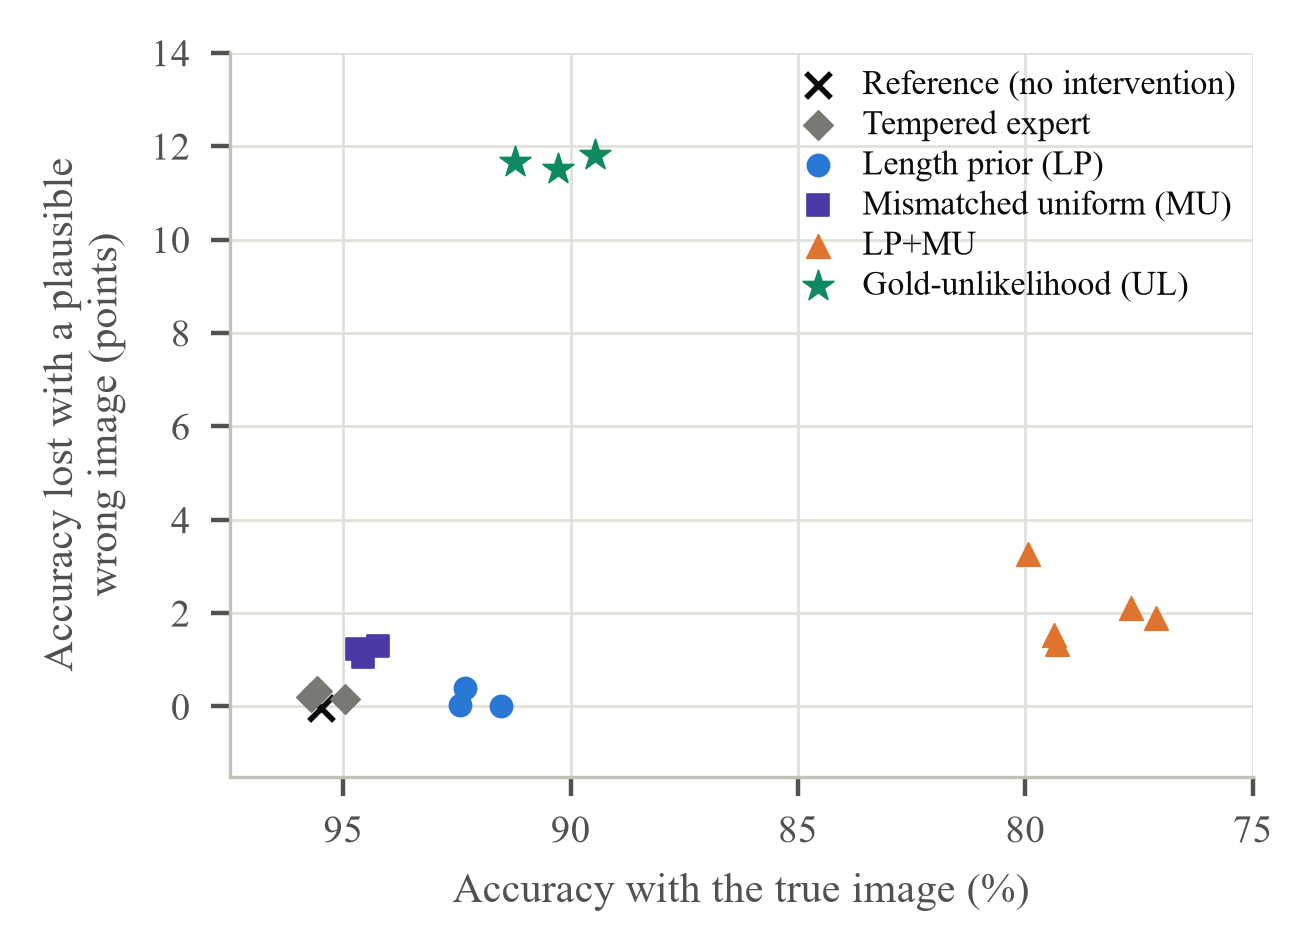
\includegraphics[width=\columnwidth]{fig/f11_price.png}
  \caption{\textbf{The price of image use on the real shortcut} (Qwen-3B, Med-CMR, 3{,}000 unseen questions, one point per run). Accuracy with the true image against the accuracy lost when the image is replaced by a plausible wrong one of the same modality; up and to the left is better.}
  \label{fig:price-supp}
\end{figure}

\paragraph{The same systems and recipe on three conditions (figure).}
\begin{figure}[h]
  \centering
  \includegraphics[width=\columnwidth]{fig/f5_two_benchmarks.pdf}
  \caption{\textbf{The same three systems and recipe on three conditions.} Orange: Med-CMR (3{,}000 unseen questions); blue: PMC-VQA (clean test, 1{,}999); violet: PMC-VQA with a length cue planted at 92\% (Sec.~5). (a)~Distribution of the black-image margin (solid, dashed, dotted: Qwen 3B, Qwen 7B, InternVL 2B). (b)~Share of predictions equal to the shortest option. (c)~Image benefit over all questions. (d)~Image benefit when the true image is blurred (radius 24 and 8\,px) or intact; mean and range over the three families.}
  \label{fig:two-supp}
\end{figure}

\paragraph{A natural dose-response, without planting anything (A42).}
Image benefit (true minus black image accuracy, points) by quintile of the text predictability of the question (option-only classifier trained on the benchmark's own training split; quintile 1 least predictable), pooled over the models of the benchmark.
\begin{center}
\footnotesize
\setlength{\tabcolsep}{3pt}
\resizebox{\linewidth}{!}{%
\begin{tabular}{@{}lcccccc@{}}
\toprule
Benchmark (questions; models) & Q1 & Q2 & Q3 & Q4 & Q5 & Spearman\\
\midrule
Med-CMR (3{,}000; 2) & $+0.3$ & 0.0 & 0.0 & 0.0 & 0.0 & $-0.71$\\
PMC-VQA (4{,}999; 3) & $+10.8$ & $+10.2$ & $+21.6$ & $+12.4$ & $+9.6$ & $-0.20$\\
OmniMedVQA (5{,}000; 3) & $+13.7$ & $+10.8$ & $+8.7$ & $+4.4$ & $+10.7$ & $-0.70$\\
A-OKVQA (1{,}145; 6) & $+35.2$ & $+33.3$ & $+40.0$ & $+34.9$ & $+34.1$ & $-0.20$\\
\bottomrule
\end{tabular}}
\end{center}
Both pre-registered rules fail (Spearman at most $-0.8$ and Q1 minus Q5 at least 5 points, each in three of four benchmarks): the largest Q1 minus Q5 difference is $+2.9$ (OmniMedVQA).
Where the blind ceiling is low the classifier's mean top probability varies only from $0.30$ to $0.51$ (PMC-VQA) and $0.30$ to $0.59$ (A-OKVQA; chance $0.25$); on Med-CMR it is $0.98$ already in the second quintile.
Limits: correlational; predictability is confounded with question type and difficulty and captures only artifacts learnable from the benchmark's training split.

\paragraph{Three things that headroom must not be confused with.}
\begin{center}
\footnotesize
\setlength{\tabcolsep}{3pt}
\resizebox{\linewidth}{!}{%
\begin{tabular}{@{}p{0.22\linewidth}p{0.36\linewidth}p{0.42\linewidth}@{}}
\toprule
Level & Tests in this paper & Status\\
\midrule
Visual information is available & every arm with the true image & given by design\\
Predictions depend on the image & black, random and plausible-wrong images; headroom; veto boundary; dose-response & tested throughout\\
The model reasons about the relevant visual content & drop under a plausible wrong image (UL: $11.6$ at 3B, $17.5$ at 7B); blur ladder (coarse identity at 3B); centre-versus-border occlusion (A-OKVQA only); judge checks (32B only) & partial; no region-level reasoning test\\
\bottomrule
\end{tabular}}
\end{center}

\paragraph{A frozen evidence-competition hypothesis for the lock-out strength (A43).}
$V$: mean over questions of $\log p(\text{gold}\mid\text{true image})-\log p(\text{gold}\mid\text{black image})$ of the cue-free ($d=0.25$) model; $S(d)=\log\frac{3d}{1-d}$ (zero at $d=0.25$); hypothesis: lock-out where $S(d^\ast)=\lambda V$, one constant $\lambda=11.1$ set on Qwen-3B/PMC-VQA.
\begin{center}
\footnotesize
\setlength{\tabcolsep}{3pt}
\resizebox{\linewidth}{!}{%
\begin{tabular}{@{}lcccc@{}}
\toprule
Condition & $V$ (nats) & predicted $S$ ($d^\ast$) & observed bracket in $d$ ($S$) & inside\\
\midrule
PMC-VQA Qwen-3B (calibration) & 0.215 & 2.39 (0.78) & 0.70--0.85 (1.95--2.83) & yes\\
PMC-VQA Qwen-7B & 0.236 & 2.62 (0.82) & 0.70--0.92 (1.95--3.54) & yes\\
PMC-VQA InternVL3-2B & 0.205 & 2.28 (0.76) & 0.70--0.92 (1.95--3.54) & yes\\
A-OKVQA Qwen-3B & 0.765 & 8.50 (0.9994) & 0.97--0.99 (4.58--5.69) & no\\
A-OKVQA Qwen-7B & 0.799 & 8.87 (0.9996) & 0.92--0.99 (3.54--5.69) & no\\
A-OKVQA InternVL3-2B & 0.987 & 10.96 (0.9999) & not locked at 0.99 & yes\\
OmniMedVQA Qwen-3B & 0.172 & 1.91 (0.69) & not locked at 0.85 & no\\
\bottomrule
\end{tabular}}
\end{center}
Inside means within 0.5 nats of the observed bracket. Rule P1 (A-OKVQA Qwen-3B) fails; P2 (three of four other conditions) holds; P3 (OmniMedVQA, prospective) fails because the prediction is already contradicted by the existing runs, so the announced runs at $d=0.92$, 0.97 and 0.99 were not performed.
P1 and P2 are retrospective (the brackets were known; only $V$ and the hypothesis were new).
The visual gain is 3.6 times larger on A-OKVQA than on PMC-VQA while the shortcut evidence at lock-out is only about 2.1 times larger, so the relation is sublinear; the hypothesis was not modified.

\paragraph{Zero-shot Qwen2.5-VL-3B next to its fine-tuned counterpart (A41).}
\begin{center}
\footnotesize
\setlength{\tabcolsep}{3pt}
\resizebox{\linewidth}{!}{%
\begin{tabular}{@{}lcccccc@{}}
\toprule
Benchmark & zero-shot true & zero-shot black & blind ceiling & ceiling $-$ black & fine-tuned black & fine-tuned $-$ zero-shot black\\
\midrule
Med-CMR & 25.6 & 23.9 & 93.7 & $+69.8$ & 95.6 & $+71.7$\\
OmniMedVQA & 74.9 & 54.0 & 94.1 & $+40.1$ & 93.2 & $+39.3$\\
PMC-VQA & 50.0 & 36.5 & 29.5 & $-7.0$ & 38.1 & $+1.7$\\
A-OKVQA & 82.8 & 49.2 & 40.1 & $-9.1$ & 49.6 & $+0.4$\\
MedXpertQA-MM & 21.3 & 21.5 & 22.9 & $+1.5$ & -- & --\\
MMMU health & 53.1 & 49.0 & 23.5 & $-25.5$ & -- & --\\
\bottomrule
\end{tabular}}
\end{center}
Rule Y1 (blind ceiling minus zero-shot black-image accuracy at least 30 points on Med-CMR and OmniMedVQA) and rule Y2 (fine-tuned minus zero-shot black-image accuracy at least 40 and 20 points) hold.
Where the benchmark has no length cue and a low blind ceiling (PMC-VQA, A-OKVQA) fine-tuning barely changes the black-image accuracy; on MMMU health the zero-shot black-image accuracy is far above the blind ceiling (the knowledge route).
The first start of this run was cancelled and is not used; the analysis script was corrected to select the complete run (documented in the amendment notes).

\paragraph{Learning curve of the shortcut (A44).}
Black-image and true-image accuracy (\%) on the 711 held-out MCQs after fine-tuning Qwen2.5-VL-3B on the first $N$ training questions (seeds 20261003 / 20261004; the A9 run for $N=9{,}277$).
\begin{center}
\footnotesize
\setlength{\tabcolsep}{3pt}
\resizebox{\linewidth}{!}{%
\begin{tabular}{@{}lccccc@{}}
\toprule
$N$ & true & black & true $-$ black & shortest option picked (true)\\
\midrule
0 (zero-shot) & 24.5 & 24.8 & $-0.3$ & 23.2\\
100 & 51.5 / 47.1 & 51.3 / 46.7 & $+0.1$ / $+0.4$ & 50.1 / 45.7\\
300 & 80.6 / 80.5 & 80.5 / 79.2 & $+0.1$ / $+1.3$ & 78.6 / 78.8\\
1{,}000 & 91.8 / 91.6 & 92.1 / 91.6 & $-0.3$ / $0.0$ & 89.2 / 88.6\\
3{,}000 & 93.8 / 94.8 & 93.8 / 94.5 & $0.0$ / $+0.3$ & 90.3 / 91.6\\
9{,}277 & 95.4 & 95.6 & $-0.3$ & 92.3\\
\bottomrule
\end{tabular}}
\end{center}
Rules L1 (black-image accuracy at least 80\% at $N=1{,}000$, both seeds), L2 (no fall of more than 2 points along $N$) and L3 (true minus black at most 2 points for every $N\ge1{,}000$) hold.
Limits: one model size and recipe, two seeds, one benchmark; the first $N$ questions are a random sample of the training order.

{
    \small
    \bibliographystyle{ieeenat_fullname}
    \bibliography{main}
}
\end{document}
